\chapter{System design}

\section{Introduction}
\section{System topology}
To ensure a suffucuent coverage it was decided to choose a system topology as shown in figure \ref{fig:tikz_system_tropology}.

\begin{figure}[h!]
	\centering
	

\tikzset{every picture/.style={line width=0.75pt}} %set default line width to 0.75pt        

\begin{tikzpicture}[x=0.75pt,y=0.75pt,yscale=-1,xscale=1]
%uncomment if require: \path (0,1074); %set diagram left start at 0, and has height of 1074

%Straight Lines [id:da776044312069671] 
\draw [color={rgb, 255:red, 155; green, 155; blue, 155 }  ,draw opacity=1 ]   (186.78,292.25) -- (186.81,286.3) ;
%Straight Lines [id:da8862888077148174] 
\draw [color={rgb, 255:red, 155; green, 155; blue, 155 }  ,draw opacity=1 ]   (181.51,294.03) -- (192.06,290.48) ;
%Shape: Rectangle [id:dp48061826630378013] 
\draw  [color={rgb, 255:red, 0; green, 41; blue, 90 }  ,draw opacity=1 ][fill={rgb, 255:red, 57; green, 107; blue, 163 }  ,fill opacity=1 ][line width=0.75]  (163.1,277.18) -- (188.58,283.72) -- (181.51,294.03) -- (156.02,287.48) -- cycle ;
%Straight Lines [id:da17291607219553407] 
\draw [color={rgb, 255:red, 0; green, 41; blue, 90 }  ,draw opacity=1 ][line width=0.75]    (162.21,278.47) -- (187.7,285.01) ;
%Straight Lines [id:da052445692069860605] 
\draw [color={rgb, 255:red, 0; green, 41; blue, 90 }  ,draw opacity=1 ][line width=0.75]    (156.91,286.2) -- (182.39,292.74) ;
%Straight Lines [id:da8572981331360381] 
\draw [color={rgb, 255:red, 0; green, 41; blue, 90 }  ,draw opacity=1 ][line width=0.75]    (157.79,284.91) -- (183.27,291.45) ;
%Straight Lines [id:da8966280462117744] 
\draw [color={rgb, 255:red, 0; green, 41; blue, 90 }  ,draw opacity=1 ][line width=0.75]    (158.68,283.62) -- (184.16,290.16) ;
%Straight Lines [id:da5157111561769883] 
\draw [color={rgb, 255:red, 0; green, 41; blue, 90 }  ,draw opacity=1 ][line width=0.75]    (161.33,279.76) -- (186.81,286.3) ;
%Straight Lines [id:da6557876795655806] 
\draw [color={rgb, 255:red, 0; green, 41; blue, 90 }  ,draw opacity=1 ][line width=0.75]    (159.56,282.33) -- (185.04,288.87) ;
%Straight Lines [id:da23526038223281698] 
\draw [color={rgb, 255:red, 0; green, 41; blue, 90 }  ,draw opacity=1 ][line width=0.75]    (160.45,281.04) -- (185.93,287.59) ;


%Straight Lines [id:da7169737054573533] 
\draw    (241,211.3) -- (211,291.3) ;
%Straight Lines [id:da07512088846003762] 
\draw    (241,211.3) -- (271,291.3) ;
%Straight Lines [id:da7109985438671316] 
\draw [color={rgb, 255:red, 0; green, 0; blue, 0 }  ,draw opacity=1 ]   (226,291.3) -- (241,266.3) ;
%Straight Lines [id:da7255851163076836] 
\draw [color={rgb, 255:red, 0; green, 0; blue, 0 }  ,draw opacity=1 ]   (256,291.3) -- (241,266.3) ;
%Straight Lines [id:da07488371271825978] 
\draw [color={rgb, 255:red, 0; green, 0; blue, 0 }  ,draw opacity=1 ]   (241,171.3) -- (241,291.3) ;
%Straight Lines [id:da5156066610561474] 
\draw    (241,186.3) -- (246,191.3) ;
%Straight Lines [id:da06286424433857807] 
\draw    (236,191.3) -- (241,186.3) ;
%Rounded Rect [id:dp32430610103781365] 
\draw  [color={rgb, 255:red, 139; green, 87; blue, 42 }  ,draw opacity=1 ][fill={rgb, 255:red, 181; green, 159; blue, 140 }  ,fill opacity=1 ] (206,287.3) .. controls (206,286.75) and (206.45,286.3) .. (207,286.3) -- (214,286.3) .. controls (214.55,286.3) and (215,286.75) .. (215,287.3) -- (215,290.3) .. controls (215,290.85) and (214.55,291.3) .. (214,291.3) -- (207,291.3) .. controls (206.45,291.3) and (206,290.85) .. (206,290.3) -- cycle ;
%Rounded Rect [id:dp887033179414831] 
\draw  [color={rgb, 255:red, 139; green, 87; blue, 42 }  ,draw opacity=1 ][fill={rgb, 255:red, 181; green, 159; blue, 140 }  ,fill opacity=1 ] (225,287.3) .. controls (225,286.75) and (225.45,286.3) .. (226,286.3) -- (233,286.3) .. controls (233.55,286.3) and (234,286.75) .. (234,287.3) -- (234,290.3) .. controls (234,290.85) and (233.55,291.3) .. (233,291.3) -- (226,291.3) .. controls (225.45,291.3) and (225,290.85) .. (225,290.3) -- cycle ;
%Rounded Rect [id:dp9630533785599515] 
\draw  [color={rgb, 255:red, 139; green, 87; blue, 42 }  ,draw opacity=1 ][fill={rgb, 255:red, 181; green, 159; blue, 140 }  ,fill opacity=1 ] (266,287.3) .. controls (266,286.75) and (266.45,286.3) .. (267,286.3) -- (274,286.3) .. controls (274.55,286.3) and (275,286.75) .. (275,287.3) -- (275,290.3) .. controls (275,290.85) and (274.55,291.3) .. (274,291.3) -- (267,291.3) .. controls (266.45,291.3) and (266,290.85) .. (266,290.3) -- cycle ;
%Rounded Rect [id:dp7607143927017899] 
\draw  [color={rgb, 255:red, 139; green, 87; blue, 42 }  ,draw opacity=1 ][fill={rgb, 255:red, 181; green, 159; blue, 140 }  ,fill opacity=1 ] (248,287.3) .. controls (248,286.75) and (248.45,286.3) .. (249,286.3) -- (256,286.3) .. controls (256.55,286.3) and (257,286.75) .. (257,287.3) -- (257,290.3) .. controls (257,290.85) and (256.55,291.3) .. (256,291.3) -- (249,291.3) .. controls (248.45,291.3) and (248,290.85) .. (248,290.3) -- cycle ;
%Straight Lines [id:da18122650418127662] 
\draw [color={rgb, 255:red, 164; green, 164; blue, 164 }  ,draw opacity=1 ][line width=1.5]    (241,156.3) -- (241,186.3) ;

%Curve Lines [id:da8766742379624342] 
\draw    (182.39,292.74) .. controls (215.75,299.93) and (222.75,289.68) .. (241,266.3) ;

%Rounded Rect [id:dp8322046966821302] 
\draw  [fill={rgb, 255:red, 235; green, 235; blue, 235 }  ,fill opacity=1 ] (517.44,332.55) .. controls (517.85,332.69) and (518.07,333.14) .. (517.92,333.55) -- (515.18,341.23) .. controls (515.03,341.64) and (514.58,341.86) .. (514.16,341.72) -- (511.92,340.96) .. controls (511.51,340.82) and (511.29,340.37) .. (511.44,339.96) -- (514.18,332.28) .. controls (514.33,331.87) and (514.78,331.65) .. (515.2,331.79) -- cycle ;
%Rounded Same Side Corner Rect [id:dp9470426755878949] 
\draw  [fill={rgb, 255:red, 184; green, 184; blue, 184 }  ,fill opacity=1 ] (514.9,342.86) .. controls (514.53,343.95) and (513.34,344.54) .. (512.25,344.19) -- (511.97,344.1) .. controls (510.88,343.74) and (510.3,342.58) .. (510.67,341.49) -- (511.76,338.32) .. controls (511.76,338.32) and (511.76,338.32) .. (511.76,338.32) -- (515.99,339.69) .. controls (515.99,339.69) and (515.99,339.69) .. (515.99,339.69) -- cycle ;
%Shape: Ellipse [id:dp07193591681477751] 
\draw  [fill={rgb, 255:red, 184; green, 184; blue, 184 }  ,fill opacity=1 ] (514.67,339.47) .. controls (515,339.15) and (515.78,339.39) .. (516.41,340.01) .. controls (517.04,340.62) and (517.29,341.38) .. (516.95,341.7) .. controls (516.62,342.02) and (515.84,341.79) .. (515.21,341.17) .. controls (514.58,340.55) and (514.34,339.79) .. (514.67,339.47) -- cycle ;

%Rounded Rect [id:dp37211141277202664] 
\draw  [fill={rgb, 255:red, 235; green, 235; blue, 235 }  ,fill opacity=1 ] (535.46,351.44) .. controls (536.07,351.45) and (536.57,351.96) .. (536.55,352.58) -- (536.39,361.32) .. controls (536.38,361.94) and (535.87,362.43) .. (535.25,362.42) -- (531.9,362.38) .. controls (531.28,362.37) and (530.79,361.86) .. (530.8,361.24) -- (530.96,352.5) .. controls (530.97,351.88) and (531.48,351.39) .. (532.1,351.4) -- cycle ;
%Snip Same Side Corner Rect [id:dp2425142825159281] 
\draw  [fill={rgb, 255:red, 184; green, 184; blue, 184 }  ,fill opacity=1 ] (530.73,362.21) -- (531.59,361.36) -- (535.57,361.36) -- (536.42,362.21) -- (536.42,363.8) -- (536.42,363.8) -- (530.73,363.8) -- (530.73,363.8) -- cycle ;
%Shape: Rectangle [id:dp31285076406775336] 
\draw  [fill={rgb, 255:red, 74; green, 74; blue, 74 }  ,fill opacity=1 ] (530.73,363.8) -- (536.42,363.8) -- (536.42,364.56) -- (530.73,364.56) -- cycle ;
%Rounded Same Side Corner Rect [id:dp8743345373509481] 
\draw  [fill={rgb, 255:red, 184; green, 184; blue, 184 }  ,fill opacity=1 ] (531.73,359.41) .. controls (531.73,359.14) and (531.95,358.92) .. (532.22,358.92) -- (534.94,358.92) .. controls (535.21,358.92) and (535.43,359.14) .. (535.43,359.41) -- (535.43,361.36) .. controls (535.43,361.36) and (535.43,361.36) .. (535.43,361.36) -- (531.73,361.36) .. controls (531.73,361.36) and (531.73,361.36) .. (531.73,361.36) -- cycle ;
%Straight Lines [id:da6591894671615994] 
\draw    (532.87,359.65) -- (534.29,359.65) ;
%Straight Lines [id:da02296919854750068] 
\draw    (532.87,360.38) -- (534.29,360.38) ;


%Rounded Rect [id:dp09742348595997496] 
\draw  [fill={rgb, 255:red, 235; green, 235; blue, 235 }  ,fill opacity=1 ] (524.15,351.74) .. controls (524.74,351.8) and (525.16,352.33) .. (525.07,352.92) -- (523.86,361.69) .. controls (523.78,362.28) and (523.23,362.7) .. (522.64,362.64) -- (519.42,362.28) .. controls (518.83,362.22) and (518.42,361.69) .. (518.5,361.1) -- (519.71,352.34) .. controls (519.79,351.75) and (520.34,351.32) .. (520.93,351.39) -- cycle ;
%Snip Same Side Corner Rect [id:dp49336996743494876] 
\draw  [fill={rgb, 255:red, 184; green, 184; blue, 184 }  ,fill opacity=1 ] (518.24,361.92) -- (519.24,361.2) -- (522.96,361.72) -- (523.66,362.69) -- (523.38,364.25) -- (523.38,364.25) -- (517.96,363.49) -- (517.96,363.49) -- cycle ;
%Shape: Rectangle [id:dp6927435968920925] 
\draw  [fill={rgb, 255:red, 74; green, 74; blue, 74 }  ,fill opacity=1 ] (517.96,363.49) -- (523.38,364.25) -- (523.24,365) -- (517.82,364.23) -- cycle ;
%Rounded Same Side Corner Rect [id:dp5660968273605633] 
\draw  [fill={rgb, 255:red, 184; green, 184; blue, 184 }  ,fill opacity=1 ] (519.68,359.28) .. controls (519.73,359.02) and (519.99,358.83) .. (520.25,358.87) -- (522.81,359.23) .. controls (523.08,359.27) and (523.25,359.51) .. (523.21,359.78) -- (522.86,361.71) .. controls (522.86,361.71) and (522.86,361.71) .. (522.86,361.71) -- (519.34,361.21) .. controls (519.34,361.21) and (519.34,361.21) .. (519.34,361.21) -- cycle ;
%Straight Lines [id:da18540275785655536] 
\draw    (520.72,359.68) -- (522.08,359.87) ;
%Straight Lines [id:da9224037321979477] 
\draw    (520.59,360.4) -- (521.95,360.59) ;


%Rounded Rect [id:dp31387605344213365] 
\draw  [fill={rgb, 255:red, 235; green, 235; blue, 235 }  ,fill opacity=1 ] (520.59,352.84) .. controls (519.92,352.71) and (519.48,352.06) .. (519.61,351.39) -- (521.72,340.85) .. controls (521.86,340.18) and (522.52,339.73) .. (523.19,339.86) -- (526.86,340.56) .. controls (527.53,340.68) and (527.97,341.33) .. (527.83,342.01) -- (525.72,352.55) .. controls (525.59,353.22) and (524.93,353.66) .. (524.26,353.53) -- cycle ;
%Rounded Rect [id:dp4024528379139658] 
\draw  [fill={rgb, 255:red, 155; green, 155; blue, 155 }  ,fill opacity=1 ] (525.56,354.33) .. controls (525.52,354.5) and (525.35,354.62) .. (525.17,354.58) -- (519.2,353.38) .. controls (519.02,353.35) and (518.91,353.18) .. (518.95,353) -- (519.15,352.04) .. controls (519.19,351.87) and (519.36,351.75) .. (519.54,351.79) -- (525.51,352.99) .. controls (525.69,353.02) and (525.8,353.19) .. (525.76,353.37) -- cycle ;
%Rounded Rect [id:dp568655330131993] 
\draw  [fill={rgb, 255:red, 235; green, 235; blue, 235 }  ,fill opacity=1 ] (535.4,352.5) .. controls (536.06,352.3) and (536.43,351.59) .. (536.22,350.93) -- (532.85,340.48) .. controls (532.64,339.82) and (531.93,339.44) .. (531.26,339.65) -- (527.63,340.75) .. controls (526.97,340.95) and (526.6,341.66) .. (526.81,342.32) -- (530.18,352.77) .. controls (530.39,353.43) and (531.11,353.81) .. (531.77,353.6) -- cycle ;
%Rounded Rect [id:dp003224129918549812] 
\draw  [fill={rgb, 255:red, 235; green, 235; blue, 235 }  ,fill opacity=1 ] (537.42,332.13) .. controls (537.57,331.73) and (538.02,331.52) .. (538.42,331.66) -- (546.36,334.39) .. controls (546.77,334.53) and (546.98,334.97) .. (546.83,335.37) -- (546.04,337.55) .. controls (545.89,337.95) and (545.45,338.16) .. (545.04,338.03) -- (537.1,335.29) .. controls (536.69,335.15) and (536.48,334.71) .. (536.63,334.31) -- cycle ;
%Rounded Same Side Corner Rect [id:dp7309919793081883] 
\draw  [fill={rgb, 255:red, 184; green, 184; blue, 184 }  ,fill opacity=1 ] (548.1,334.69) .. controls (549.16,335.04) and (549.73,336.19) .. (549.36,337.25) -- (549.26,337.52) .. controls (548.89,338.57) and (547.73,339.15) .. (546.66,338.79) -- (543.32,337.69) .. controls (543.32,337.69) and (543.32,337.69) .. (543.32,337.69) -- (544.75,333.59) .. controls (544.75,333.59) and (544.75,333.59) .. (544.75,333.59) -- cycle ;
%Shape: Ellipse [id:dp2264261851201852] 
\draw  [fill={rgb, 255:red, 184; green, 184; blue, 184 }  ,fill opacity=1 ] (544.52,334.87) .. controls (544.19,334.54) and (544.44,333.78) .. (545.08,333.17) .. controls (545.72,332.56) and (546.5,332.33) .. (546.83,332.66) .. controls (547.16,332.98) and (546.91,333.74) .. (546.27,334.35) .. controls (545.63,334.96) and (544.85,335.19) .. (544.52,334.87) -- cycle ;
%Rounded Rect [id:dp564252146824956] 
\draw  [fill={rgb, 255:red, 235; green, 235; blue, 235 }  ,fill opacity=1 ] (519.57,323.6) .. controls (519.57,321.94) and (520.92,320.58) .. (522.59,320.58) -- (531.65,320.58) .. controls (533.32,320.58) and (534.67,321.94) .. (534.67,323.6) -- (534.67,336.16) .. controls (534.67,337.83) and (533.32,339.18) .. (531.65,339.18) -- (522.59,339.18) .. controls (520.92,339.18) and (519.57,337.83) .. (519.57,336.16) -- cycle ;
%Rounded Rect [id:dp2787395635949117] 
\draw  [fill={rgb, 255:red, 235; green, 235; blue, 235 }  ,fill opacity=1 ] (525.28,328.25) .. controls (525.62,328.68) and (525.53,329.3) .. (525.09,329.63) -- (517.92,334.93) .. controls (517.47,335.26) and (516.84,335.17) .. (516.5,334.73) -- (514.65,332.37) .. controls (514.31,331.93) and (514.4,331.31) .. (514.84,330.98) -- (522.01,325.69) .. controls (522.46,325.36) and (523.09,325.45) .. (523.43,325.88) -- cycle ;
%Rounded Rect [id:dp786297812306815] 
\draw  [fill={rgb, 255:red, 235; green, 235; blue, 235 }  ,fill opacity=1 ] (530.86,326.27) .. controls (531.2,325.83) and (531.84,325.75) .. (532.28,326.07) -- (539.45,331.38) .. controls (539.9,331.7) and (539.98,332.32) .. (539.64,332.76) -- (537.79,335.12) .. controls (537.45,335.56) and (536.82,335.64) .. (536.37,335.31) -- (529.2,330.01) .. controls (528.76,329.69) and (528.68,329.07) .. (529.02,328.63) -- cycle ;
%Shape: Ellipse [id:dp7124593520753895] 
\draw  [fill={rgb, 255:red, 235; green, 235; blue, 235 }  ,fill opacity=1 ] (527.15,324.54) .. controls (530.61,324.54) and (533.42,328.91) .. (533.42,334.3) .. controls (533.42,339.69) and (530.61,344.06) .. (527.15,344.06) .. controls (523.68,344.06) and (520.87,339.69) .. (520.87,334.3) .. controls (520.87,328.91) and (523.68,324.54) .. (527.15,324.54) -- cycle ;
%Rounded Rect [id:dp5813009502758648] 
\draw  [fill={rgb, 255:red, 235; green, 235; blue, 235 }  ,fill opacity=1 ] (520.87,338.69) .. controls (520.87,338.29) and (521.2,337.96) .. (521.61,337.96) -- (532.69,337.96) .. controls (533.09,337.96) and (533.42,338.29) .. (533.42,338.69) -- (533.42,340.89) .. controls (533.42,341.29) and (533.09,341.62) .. (532.69,341.62) -- (521.61,341.62) .. controls (521.2,341.62) and (520.87,341.29) .. (520.87,340.89) -- cycle ;
%Straight Lines [id:da9843916595094087] 
\draw [color={rgb, 255:red, 128; green, 128; blue, 128 }  ,draw opacity=1 ]   (527.15,339.18) -- (527.15,340.4) ;
%Straight Lines [id:da44278050658443013] 
\draw [color={rgb, 255:red, 128; green, 128; blue, 128 }  ,draw opacity=1 ]   (525.89,339.18) -- (525.89,340.4) ;
%Straight Lines [id:da8515923429999195] 
\draw [color={rgb, 255:red, 128; green, 128; blue, 128 }  ,draw opacity=1 ]   (524.64,339.18) -- (524.64,340.4) ;
%Straight Lines [id:da33036684979989395] 
\draw [color={rgb, 255:red, 128; green, 128; blue, 128 }  ,draw opacity=1 ]   (523.38,339.18) -- (523.38,340.4) ;
%Straight Lines [id:da1593271076470817] 
\draw [color={rgb, 255:red, 128; green, 128; blue, 128 }  ,draw opacity=1 ]   (522.13,339.18) -- (522.13,340.4) ;
%Shape: Ellipse [id:dp9202045909077847] 
\draw  [fill={rgb, 255:red, 155; green, 155; blue, 155 }  ,fill opacity=1 ] (528.4,339.79) .. controls (528.4,339.45) and (528.68,339.18) .. (529.03,339.18) .. controls (529.37,339.18) and (529.65,339.45) .. (529.65,339.79) .. controls (529.65,340.13) and (529.37,340.4) .. (529.03,340.4) .. controls (528.68,340.4) and (528.4,340.13) .. (528.4,339.79) -- cycle ;
%Shape: Ellipse [id:dp7271752923032224] 
\draw  [fill={rgb, 255:red, 155; green, 155; blue, 155 }  ,fill opacity=1 ] (530.91,339.79) .. controls (530.91,339.45) and (531.19,339.18) .. (531.54,339.18) .. controls (531.88,339.18) and (532.16,339.45) .. (532.16,339.79) .. controls (532.16,340.13) and (531.88,340.4) .. (531.54,340.4) .. controls (531.19,340.4) and (530.91,340.13) .. (530.91,339.79) -- cycle ;

%Rounded Rect [id:dp6720029784684363] 
\draw  [fill={rgb, 255:red, 155; green, 155; blue, 155 }  ,fill opacity=1 ] (514.06,331.52) .. controls (514.16,331.38) and (514.36,331.35) .. (514.5,331.45) -- (518.68,334.44) .. controls (518.82,334.54) and (518.85,334.73) .. (518.75,334.87) -- (518.18,335.61) .. controls (518.08,335.75) and (517.88,335.78) .. (517.74,335.68) -- (513.56,332.69) .. controls (513.42,332.59) and (513.39,332.4) .. (513.49,332.26) -- cycle ;
%Rounded Rect [id:dp027930408219279945] 
\draw  [fill={rgb, 255:red, 155; green, 155; blue, 155 }  ,fill opacity=1 ] (540.71,331.47) .. controls (540.86,331.56) and (540.9,331.75) .. (540.81,331.9) -- (538.11,336.2) .. controls (538.01,336.34) and (537.82,336.39) .. (537.67,336.3) -- (536.86,335.82) .. controls (536.71,335.73) and (536.66,335.54) .. (536.75,335.39) -- (539.46,331.1) .. controls (539.55,330.95) and (539.75,330.9) .. (539.89,330.99) -- cycle ;
%Rounded Rect [id:dp8813279022887199] 
\draw  [fill={rgb, 255:red, 155; green, 155; blue, 155 }  ,fill opacity=1 ] (536.9,352.36) .. controls (536.95,352.53) and (536.84,352.71) .. (536.67,352.76) -- (530.79,354.33) .. controls (530.62,354.38) and (530.44,354.28) .. (530.39,354.1) -- (530.12,353.16) .. controls (530.07,352.99) and (530.18,352.81) .. (530.35,352.77) -- (536.23,351.19) .. controls (536.4,351.14) and (536.58,351.25) .. (536.63,351.42) -- cycle ;
%Image [id:dp9572506042729121] 
\draw (527.15,333.07) node  {
\includegraphics[width=8.47pt,height=5.08pt]{images/image_oewf_logo}};
%Straight Lines [id:da4534725400264392] 
\draw [color={rgb, 255:red, 128; green, 128; blue, 128 }  ,draw opacity=1 ]   (531.78,316.35) -- (531.78,319.61) ;
%Straight Lines [id:da8847913013765427] 
\draw [color={rgb, 255:red, 0; green, 0; blue, 0 }  ,draw opacity=1 ]   (530.67,314.18) -- (530.67,318.53) ;
%Straight Lines [id:da22865458397103677] 
\draw [color={rgb, 255:red, 0; green, 0; blue, 0 }  ,draw opacity=1 ]   (524.01,314.18) -- (524.01,318.53) ;
%Shape: Ellipse [id:dp3200368331258012] 
\draw  [color={rgb, 255:red, 0; green, 0; blue, 0 }  ,draw opacity=1 ][fill={rgb, 255:red, 235; green, 235; blue, 235 }  ,fill opacity=1 ] (521.79,322.87) .. controls (521.79,319.87) and (524.27,317.44) .. (527.34,317.44) .. controls (530.4,317.44) and (532.89,319.87) .. (532.89,322.87) .. controls (532.89,325.87) and (530.4,328.3) .. (527.34,328.3) .. controls (524.27,328.3) and (521.79,325.87) .. (521.79,322.87) -- cycle ;
%Shape: Ellipse [id:dp5175787135463579] 
\draw  [fill={rgb, 255:red, 255; green, 213; blue, 144 }  ,fill opacity=1 ] (521.91,322.87) .. controls (521.91,321.19) and (524.34,319.83) .. (527.34,319.83) .. controls (530.34,319.83) and (532.77,321.19) .. (532.77,322.87) .. controls (532.77,324.55) and (530.34,325.91) .. (527.34,325.91) .. controls (524.34,325.91) and (521.91,324.55) .. (521.91,322.87) -- cycle ;
%Shape: Ellipse [id:dp26487190585460096] 
\draw  [fill={rgb, 255:red, 255; green, 246; blue, 136 }  ,fill opacity=1 ] (522.05,319.2) .. controls (522.05,318.85) and (522.34,318.57) .. (522.7,318.57) .. controls (523.05,318.57) and (523.34,318.85) .. (523.34,319.2) .. controls (523.34,319.55) and (523.05,319.83) .. (522.7,319.83) .. controls (522.34,319.83) and (522.05,319.55) .. (522.05,319.2) -- cycle ;
%Curve Lines [id:da2116343907025895] 
\draw [color={rgb, 255:red, 248; green, 231; blue, 28 }  ,draw opacity=1 ]   (530.86,324.07) .. controls (531.46,323.34) and (531.53,322.55) .. (530.86,321.75) ;
%Curve Lines [id:da28329089162972054] 
\draw [color={rgb, 255:red, 248; green, 231; blue, 28 }  ,draw opacity=1 ]   (529.9,323.99) .. controls (530.49,323.27) and (530.57,322.47) .. (529.9,321.68) ;

%Rounded Rect [id:dp8037695527260584] 
\draw  [fill={rgb, 255:red, 235; green, 235; blue, 235 }  ,fill opacity=1 ] (409.25,313.74) .. controls (409.68,313.77) and (410.01,314.15) .. (409.98,314.59) -- (409.39,322.69) .. controls (409.36,323.13) and (408.98,323.46) .. (408.54,323.43) -- (406.17,323.26) .. controls (405.73,323.23) and (405.4,322.85) .. (405.44,322.42) -- (406.03,314.32) .. controls (406.06,313.88) and (406.44,313.55) .. (406.88,313.58) -- cycle ;
%Rounded Same Side Corner Rect [id:dp21637858049510905] 
\draw  [fill={rgb, 255:red, 184; green, 184; blue, 184 }  ,fill opacity=1 ] (409.55,324.33) .. controls (409.49,325.48) and (408.5,326.36) .. (407.35,326.29) -- (407.06,326.28) .. controls (405.91,326.21) and (405.04,325.23) .. (405.11,324.08) -- (405.31,320.75) .. controls (405.31,320.75) and (405.31,320.75) .. (405.31,320.75) -- (409.76,321) .. controls (409.76,321) and (409.76,321) .. (409.76,321) -- cycle ;
%Shape: Ellipse [id:dp2891636717279016] 
\draw  [fill={rgb, 255:red, 184; green, 184; blue, 184 }  ,fill opacity=1 ] (408.43,321.13) .. controls (408.66,320.73) and (409.48,320.77) .. (410.25,321.2) .. controls (411.03,321.64) and (411.46,322.31) .. (411.23,322.71) .. controls (411,323.1) and (410.18,323.06) .. (409.4,322.63) .. controls (408.63,322.19) and (408.19,321.52) .. (408.43,321.13) -- cycle ;

%Rounded Rect [id:dp18937263124579817] 
\draw  [fill={rgb, 255:red, 235; green, 235; blue, 235 }  ,fill opacity=1 ] (415.31,331.86) .. controls (415.92,331.91) and (416.36,332.43) .. (416.31,333.04) -- (415.46,341.79) .. controls (415.4,342.39) and (414.86,342.85) .. (414.25,342.8) -- (410.95,342.56) .. controls (410.35,342.52) and (409.9,341.99) .. (409.96,341.38) -- (410.81,332.63) .. controls (410.87,332.03) and (411.41,331.57) .. (412.02,331.62) -- cycle ;
%Snip Same Side Corner Rect [id:dp6616884714452531] 
\draw  [fill={rgb, 255:red, 184; green, 184; blue, 184 }  ,fill opacity=1 ] (409.82,342.33) -- (410.74,341.53) -- (414.63,341.76) -- (415.42,342.66) -- (415.29,344.25) -- (415.29,344.25) -- (409.7,343.91) -- (409.7,343.91) -- cycle ;
%Shape: Rectangle [id:dp15631152692673145] 
\draw  [fill={rgb, 255:red, 74; green, 74; blue, 74 }  ,fill opacity=1 ] (409.7,343.91) -- (415.29,344.24) -- (415.23,345) -- (409.64,344.67) -- cycle ;
%Rounded Same Side Corner Rect [id:dp6825995668168245] 
\draw  [fill={rgb, 255:red, 184; green, 184; blue, 184 }  ,fill opacity=1 ] (411.02,339.59) .. controls (411.04,339.32) and (411.28,339.11) .. (411.55,339.13) -- (414.21,339.29) .. controls (414.48,339.3) and (414.68,339.54) .. (414.66,339.8) -- (414.51,341.75) .. controls (414.51,341.75) and (414.51,341.75) .. (414.51,341.75) -- (410.87,341.54) .. controls (410.87,341.54) and (410.87,341.54) .. (410.87,341.54) -- cycle ;
%Straight Lines [id:da7834095127019931] 
\draw    (412.12,339.9) -- (413.52,339.98) ;
%Straight Lines [id:da43426943250078387] 
\draw    (412.07,340.63) -- (413.46,340.71) ;


%Rounded Rect [id:dp12524116124979567] 
\draw  [fill={rgb, 255:red, 235; green, 235; blue, 235 }  ,fill opacity=1 ] (426.51,331.69) .. controls (427.1,331.69) and (427.57,332.17) .. (427.57,332.76) -- (427.52,341.61) .. controls (427.52,342.19) and (427.04,342.67) .. (426.45,342.67) -- (423.24,342.65) .. controls (422.65,342.65) and (422.18,342.17) .. (422.18,341.58) -- (422.23,332.74) .. controls (422.23,332.15) and (422.71,331.67) .. (423.3,331.67) -- cycle ;
%Snip Same Side Corner Rect [id:dp9377315892028506] 
\draw  [fill={rgb, 255:red, 184; green, 184; blue, 184 }  ,fill opacity=1 ] (422.03,342.41) -- (422.92,341.59) -- (426.64,341.73) -- (427.45,342.61) -- (427.38,344.2) -- (427.38,344.2) -- (421.96,344) -- (421.96,344) -- cycle ;
%Shape: Rectangle [id:dp9480931961962293] 
\draw  [fill={rgb, 255:red, 74; green, 74; blue, 74 }  ,fill opacity=1 ] (421.96,344) -- (427.38,344.2) -- (427.35,344.95) -- (421.93,344.75) -- cycle ;
%Rounded Same Side Corner Rect [id:dp4729725698374143] 
\draw  [fill={rgb, 255:red, 184; green, 184; blue, 184 }  ,fill opacity=1 ] (423.11,339.64) .. controls (423.12,339.38) and (423.35,339.16) .. (423.62,339.17) -- (426.16,339.27) .. controls (426.43,339.28) and (426.64,339.5) .. (426.63,339.77) -- (426.54,341.72) .. controls (426.54,341.72) and (426.54,341.72) .. (426.54,341.72) -- (423.02,341.59) .. controls (423.02,341.59) and (423.02,341.59) .. (423.02,341.59) -- cycle ;
%Straight Lines [id:da41492353454429076] 
\draw    (424.18,339.93) -- (425.54,339.98) ;
%Straight Lines [id:da5104594908219127] 
\draw    (424.15,340.66) -- (425.5,340.71) ;


%Rounded Rect [id:dp3828926464084914] 
\draw  [fill={rgb, 255:red, 235; green, 235; blue, 235 }  ,fill opacity=1 ] (411.79,332.8) .. controls (411.11,332.67) and (410.67,332.02) .. (410.81,331.35) -- (412.91,320.84) .. controls (413.05,320.17) and (413.71,319.73) .. (414.38,319.85) -- (418.05,320.55) .. controls (418.72,320.68) and (419.16,321.33) .. (419.02,322) -- (416.92,332.51) .. controls (416.78,333.18) and (416.13,333.62) .. (415.45,333.49) -- cycle ;
%Rounded Rect [id:dp6814403537537304] 
\draw  [fill={rgb, 255:red, 155; green, 155; blue, 155 }  ,fill opacity=1 ] (416.85,334.22) .. controls (416.81,334.4) and (416.64,334.51) .. (416.46,334.48) -- (410.49,333.28) .. controls (410.31,333.24) and (410.2,333.07) .. (410.24,332.89) -- (410.44,331.94) .. controls (410.48,331.76) and (410.65,331.65) .. (410.83,331.68) -- (416.8,332.88) .. controls (416.98,332.92) and (417.09,333.09) .. (417.05,333.26) -- cycle ;
%Rounded Rect [id:dp898968778923305] 
\draw  [fill={rgb, 255:red, 235; green, 235; blue, 235 }  ,fill opacity=1 ] (426.56,332.42) .. controls (427.23,332.21) and (427.6,331.51) .. (427.38,330.85) -- (424.04,320.47) .. controls (423.83,319.81) and (423.12,319.44) .. (422.45,319.64) -- (418.82,320.74) .. controls (418.16,320.95) and (417.79,321.65) .. (418,322.31) -- (421.34,332.69) .. controls (421.56,333.35) and (422.27,333.72) .. (422.94,333.52) -- cycle ;
%Rounded Rect [id:dp1467174660270889] 
\draw  [fill={rgb, 255:red, 235; green, 235; blue, 235 }  ,fill opacity=1 ] (429.61,313.45) .. controls (430.02,313.31) and (430.47,313.53) .. (430.62,313.94) -- (433.43,321.6) .. controls (433.58,322.01) and (433.37,322.46) .. (432.95,322.6) -- (430.71,323.37) .. controls (430.3,323.52) and (429.85,323.3) .. (429.7,322.89) -- (426.89,315.23) .. controls (426.74,314.82) and (426.95,314.37) .. (427.37,314.23) -- cycle ;
%Rounded Same Side Corner Rect [id:dp9343258349727852] 
\draw  [fill={rgb, 255:red, 184; green, 184; blue, 184 }  ,fill opacity=1 ] (434.26,323.05) .. controls (434.67,324.12) and (434.13,325.3) .. (433.05,325.69) -- (432.78,325.79) .. controls (431.7,326.17) and (430.49,325.62) .. (430.09,324.55) -- (428.89,321.41) .. controls (428.89,321.41) and (428.89,321.41) .. (428.89,321.41) -- (433.07,319.9) .. controls (433.07,319.9) and (433.07,319.9) .. (433.07,319.9) -- cycle ;
%Shape: Ellipse [id:dp3065499685960065] 
\draw  [fill={rgb, 255:red, 184; green, 184; blue, 184 }  ,fill opacity=1 ] (429.41,321.28) .. controls (429.86,321.42) and (430,322.2) .. (429.74,323.03) .. controls (429.47,323.86) and (428.9,324.43) .. (428.45,324.29) .. controls (428,324.16) and (427.86,323.37) .. (428.12,322.54) .. controls (428.39,321.71) and (428.96,321.15) .. (429.41,321.28) -- cycle ;
%Rounded Rect [id:dp9551012915692443] 
\draw  [fill={rgb, 255:red, 235; green, 235; blue, 235 }  ,fill opacity=1 ] (410.76,303.6) .. controls (410.76,301.93) and (412.11,300.58) .. (413.78,300.58) -- (422.84,300.58) .. controls (424.51,300.58) and (425.86,301.93) .. (425.86,303.6) -- (425.86,316.15) .. controls (425.86,317.82) and (424.51,319.17) .. (422.84,319.17) -- (413.78,319.17) .. controls (412.11,319.17) and (410.76,317.82) .. (410.76,316.15) -- cycle ;
%Rounded Rect [id:dp15819031862520028] 
\draw  [fill={rgb, 255:red, 235; green, 235; blue, 235 }  ,fill opacity=1 ] (416.17,308.6) .. controls (416.59,308.96) and (416.63,309.59) .. (416.25,310) -- (410.28,316.53) .. controls (409.9,316.94) and (409.26,316.97) .. (408.84,316.61) -- (406.56,314.64) .. controls (406.14,314.27) and (406.1,313.64) .. (406.48,313.24) -- (412.45,306.71) .. controls (412.83,306.3) and (413.47,306.26) .. (413.89,306.62) -- cycle ;
%Rounded Rect [id:dp5408558056429151] 
\draw  [fill={rgb, 255:red, 155; green, 155; blue, 155 }  ,fill opacity=1 ] (405.79,313.46) .. controls (405.88,313.31) and (406.08,313.27) .. (406.23,313.36) -- (410.6,316.08) .. controls (410.75,316.17) and (410.79,316.36) .. (410.7,316.5) -- (410.18,317.29) .. controls (410.09,317.43) and (409.89,317.47) .. (409.75,317.38) -- (405.37,314.66) .. controls (405.23,314.57) and (405.18,314.38) .. (405.28,314.24) -- cycle ;
%Rounded Rect [id:dp1563472198552185] 
\draw  [fill={rgb, 255:red, 235; green, 235; blue, 235 }  ,fill opacity=1 ] (422.5,306.55) .. controls (422.91,306.19) and (423.56,306.22) .. (423.94,306.62) -- (429.98,313.09) .. controls (430.36,313.5) and (430.33,314.13) .. (429.91,314.49) -- (427.65,316.49) .. controls (427.23,316.86) and (426.59,316.83) .. (426.21,316.42) -- (420.17,309.95) .. controls (419.79,309.55) and (419.82,308.92) .. (420.24,308.55) -- cycle ;
%Rounded Rect [id:dp22465164770492918] 
\draw  [fill={rgb, 255:red, 155; green, 155; blue, 155 }  ,fill opacity=1 ] (431.23,313.82) .. controls (431.35,313.94) and (431.35,314.14) .. (431.23,314.25) -- (427.51,317.77) .. controls (427.38,317.89) and (427.18,317.89) .. (427.06,317.77) -- (426.4,317.1) .. controls (426.28,316.98) and (426.28,316.78) .. (426.4,316.67) -- (430.12,313.15) .. controls (430.25,313.03) and (430.45,313.03) .. (430.57,313.15) -- cycle ;
%Shape: Ellipse [id:dp7977007467753716] 
\draw  [fill={rgb, 255:red, 235; green, 235; blue, 235 }  ,fill opacity=1 ] (418.34,304.53) .. controls (421.8,304.53) and (424.61,308.9) .. (424.61,314.29) .. controls (424.61,319.68) and (421.8,324.05) .. (418.34,324.05) .. controls (414.87,324.05) and (412.06,319.68) .. (412.06,314.29) .. controls (412.06,308.9) and (414.87,304.53) .. (418.34,304.53) -- cycle ;
%Rounded Rect [id:dp8358614393968633] 
\draw  [fill={rgb, 255:red, 235; green, 235; blue, 235 }  ,fill opacity=1 ] (412.06,318.68) .. controls (412.06,318.28) and (412.39,317.95) .. (412.8,317.95) -- (423.88,317.95) .. controls (424.28,317.95) and (424.61,318.28) .. (424.61,318.68) -- (424.61,320.88) .. controls (424.61,321.29) and (424.28,321.61) .. (423.88,321.61) -- (412.8,321.61) .. controls (412.39,321.61) and (412.06,321.29) .. (412.06,320.88) -- cycle ;
%Straight Lines [id:da8363176964830652] 
\draw [color={rgb, 255:red, 128; green, 128; blue, 128 }  ,draw opacity=1 ]   (418.34,319.17) -- (418.34,320.39) ;
%Straight Lines [id:da721704331754992] 
\draw [color={rgb, 255:red, 128; green, 128; blue, 128 }  ,draw opacity=1 ]   (417.08,319.17) -- (417.08,320.39) ;
%Straight Lines [id:da9125880632893739] 
\draw [color={rgb, 255:red, 128; green, 128; blue, 128 }  ,draw opacity=1 ]   (415.83,319.17) -- (415.83,320.39) ;
%Straight Lines [id:da36419010739606206] 
\draw [color={rgb, 255:red, 128; green, 128; blue, 128 }  ,draw opacity=1 ]   (414.57,319.17) -- (414.57,320.39) ;
%Straight Lines [id:da7608541801523907] 
\draw [color={rgb, 255:red, 128; green, 128; blue, 128 }  ,draw opacity=1 ]   (413.32,319.17) -- (413.32,320.39) ;
%Shape: Ellipse [id:dp585957770231951] 
\draw  [fill={rgb, 255:red, 155; green, 155; blue, 155 }  ,fill opacity=1 ] (419.59,319.78) .. controls (419.59,319.45) and (419.87,319.17) .. (420.22,319.17) .. controls (420.56,319.17) and (420.84,319.45) .. (420.84,319.78) .. controls (420.84,320.12) and (420.56,320.39) .. (420.22,320.39) .. controls (419.87,320.39) and (419.59,320.12) .. (419.59,319.78) -- cycle ;
%Shape: Ellipse [id:dp2164375054096188] 
\draw  [fill={rgb, 255:red, 155; green, 155; blue, 155 }  ,fill opacity=1 ] (422.1,319.78) .. controls (422.1,319.45) and (422.38,319.17) .. (422.73,319.17) .. controls (423.07,319.17) and (423.35,319.45) .. (423.35,319.78) .. controls (423.35,320.12) and (423.07,320.39) .. (422.73,320.39) .. controls (422.38,320.39) and (422.1,320.12) .. (422.1,319.78) -- cycle ;

%Rounded Rect [id:dp47069113285328035] 
\draw  [fill={rgb, 255:red, 155; green, 155; blue, 155 }  ,fill opacity=1 ] (428.17,332.43) .. controls (428.22,332.61) and (428.12,332.78) .. (427.94,332.83) -- (422.07,334.41) .. controls (421.89,334.45) and (421.71,334.35) .. (421.66,334.18) -- (421.4,333.24) .. controls (421.35,333.06) and (421.45,332.89) .. (421.62,332.84) -- (427.5,331.26) .. controls (427.67,331.22) and (427.86,331.32) .. (427.9,331.49) -- cycle ;
%Image [id:dp1573253290255252] 
\draw (418.34,313.07) node  {
\includegraphics[width=8.47pt,height=5.08pt]{images/image_oewf_logo}};
%Straight Lines [id:da7451230208262558] 
\draw [color={rgb, 255:red, 128; green, 128; blue, 128 }  ,draw opacity=1 ]   (422.59,296.63) -- (422.59,299.89) ;
%Straight Lines [id:da6255085722787601] 
\draw [color={rgb, 255:red, 0; green, 0; blue, 0 }  ,draw opacity=1 ]   (421.48,294.46) -- (421.48,298.8) ;
%Straight Lines [id:da7722232170950842] 
\draw [color={rgb, 255:red, 0; green, 0; blue, 0 }  ,draw opacity=1 ]   (414.82,294.46) -- (414.82,298.8) ;
%Shape: Ellipse [id:dp30109204748682883] 
\draw  [color={rgb, 255:red, 0; green, 0; blue, 0 }  ,draw opacity=1 ][fill={rgb, 255:red, 235; green, 235; blue, 235 }  ,fill opacity=1 ] (412.6,303.15) .. controls (412.6,300.15) and (415.09,297.72) .. (418.15,297.72) .. controls (421.22,297.72) and (423.7,300.15) .. (423.7,303.15) .. controls (423.7,306.15) and (421.22,308.58) .. (418.15,308.58) .. controls (415.09,308.58) and (412.6,306.15) .. (412.6,303.15) -- cycle ;
%Shape: Ellipse [id:dp4478388996828948] 
\draw  [fill={rgb, 255:red, 255; green, 213; blue, 144 }  ,fill opacity=1 ] (412.72,303.15) .. controls (412.72,301.47) and (415.15,300.11) .. (418.15,300.11) .. controls (421.15,300.11) and (423.58,301.47) .. (423.58,303.15) .. controls (423.58,304.83) and (421.15,306.19) .. (418.15,306.19) .. controls (415.15,306.19) and (412.72,304.83) .. (412.72,303.15) -- cycle ;
%Shape: Ellipse [id:dp6630674107274876] 
\draw  [fill={rgb, 255:red, 255; green, 246; blue, 136 }  ,fill opacity=1 ] (412.87,299.48) .. controls (412.87,299.13) and (413.15,298.85) .. (413.51,298.85) .. controls (413.87,298.85) and (414.15,299.13) .. (414.15,299.48) .. controls (414.15,299.83) and (413.87,300.11) .. (413.51,300.11) .. controls (413.15,300.11) and (412.87,299.83) .. (412.87,299.48) -- cycle ;
%Curve Lines [id:da5193068235721494] 
\draw [color={rgb, 255:red, 248; green, 231; blue, 28 }  ,draw opacity=1 ]   (421.68,304.34) .. controls (422.27,303.62) and (422.34,302.82) .. (421.68,302.03) ;
%Curve Lines [id:da926198929702498] 
\draw [color={rgb, 255:red, 248; green, 231; blue, 28 }  ,draw opacity=1 ]   (420.71,304.27) .. controls (421.31,303.55) and (421.38,302.75) .. (420.71,301.95) ;

%Straight Lines [id:da00769059166381969] 
\draw [color={rgb, 255:red, 0; green, 0; blue, 0 }  ,draw opacity=1 ]   (70,200) -- (75,185) ;
%Straight Lines [id:da46598579370706616] 
\draw [color={rgb, 255:red, 0; green, 0; blue, 0 }  ,draw opacity=1 ]   (80,200) -- (75,185) ;
%Straight Lines [id:da23709980119101592] 
\draw [color={rgb, 255:red, 0; green, 0; blue, 0 }  ,draw opacity=1 ]   (75,170) -- (75,200) ;
%Rounded Rect [id:dp7878838006003148] 
\draw  [fill={rgb, 255:red, 229; green, 229; blue, 229 }  ,fill opacity=1 ] (25,208) .. controls (25,203.58) and (28.58,200) .. (33,200) -- (82,200) .. controls (86.42,200) and (90,203.58) .. (90,208) -- (90,232) .. controls (90,236.42) and (86.42,240) .. (82,240) -- (33,240) .. controls (28.58,240) and (25,236.42) .. (25,232) -- cycle ;
%Rounded Rect [id:dp009643529528236439] 
\draw  [fill={rgb, 255:red, 179; green, 179; blue, 179 }  ,fill opacity=1 ] (30,208) .. controls (30,206.34) and (31.34,205) .. (33,205) -- (42,205) .. controls (43.66,205) and (45,206.34) .. (45,208) -- (45,232) .. controls (45,233.66) and (43.66,235) .. (42,235) -- (33,235) .. controls (31.34,235) and (30,233.66) .. (30,232) -- cycle ;
%Shape: Circle [id:dp7916078516717486] 
\draw  [fill={rgb, 255:red, 190; green, 215; blue, 246 }  ,fill opacity=1 ] (35,212.5) .. controls (35,211.12) and (36.12,210) .. (37.5,210) .. controls (38.88,210) and (40,211.12) .. (40,212.5) .. controls (40,213.88) and (38.88,215) .. (37.5,215) .. controls (36.12,215) and (35,213.88) .. (35,212.5) -- cycle ;

%Rounded Rect [id:dp27829438729336387] 
\draw  [fill={rgb, 255:red, 190; green, 215; blue, 246 }  ,fill opacity=1 ] (50,208) .. controls (50,206.34) and (51.34,205) .. (53,205) -- (62,205) .. controls (63.66,205) and (65,206.34) .. (65,208) -- (65,217) .. controls (65,218.66) and (63.66,220) .. (62,220) -- (53,220) .. controls (51.34,220) and (50,218.66) .. (50,217) -- cycle ;
%Rounded Rect [id:dp6191699287037458] 
\draw  [fill={rgb, 255:red, 190; green, 215; blue, 246 }  ,fill opacity=1 ] (70,208) .. controls (70,206.34) and (71.34,205) .. (73,205) -- (82,205) .. controls (83.66,205) and (85,206.34) .. (85,208) -- (85,217) .. controls (85,218.66) and (83.66,220) .. (82,220) -- (73,220) .. controls (71.34,220) and (70,218.66) .. (70,217) -- cycle ;
%Straight Lines [id:da6770638771918465] 
\draw    (75,175) -- (80,180) ;
%Straight Lines [id:da8659188665790745] 
\draw    (75,175) -- (70,180) ;
%Straight Lines [id:da2564512721112855] 
\draw [color={rgb, 255:red, 164; green, 164; blue, 164 }  ,draw opacity=1 ][line width=1.5]    (75,145) -- (75,175) ;
%Image [id:dp6702525874715359] 
\draw (67.65,229.63) node  {
\includegraphics[width=18.38pt,height=10.69pt]{images/image_oewf_logo}};

%Straight Lines [id:da852327524129781] 
\draw [color={rgb, 255:red, 101; green, 162; blue, 30 }  ,draw opacity=1 ]   (253.94,175.49) -- (368.06,204.51) ;
\draw [shift={(370,205)}, rotate = 194.26] [color={rgb, 255:red, 101; green, 162; blue, 30 }  ,draw opacity=1 ][line width=0.75]    (10.93,-3.29) .. controls (6.95,-1.4) and (3.31,-0.3) .. (0,0) .. controls (3.31,0.3) and (6.95,1.4) .. (10.93,3.29)   ;
\draw [shift={(252,175)}, rotate = 14.26] [color={rgb, 255:red, 101; green, 162; blue, 30 }  ,draw opacity=1 ][line width=0.75]    (10.93,-3.29) .. controls (6.95,-1.4) and (3.31,-0.3) .. (0,0) .. controls (3.31,0.3) and (6.95,1.4) .. (10.93,3.29)   ;
%Shape: Trapezoid [id:dp9492548671397596] 
\draw  [color={rgb, 255:red, 178; green, 111; blue, 0 }  ,draw opacity=1 ][fill={rgb, 255:red, 245; green, 166; blue, 35 }  ,fill opacity=1 ] (120.62,349.66) -- (119.18,350.09) -- (119.18,352.12) -- (120.62,352.55) -- cycle ;
%Shape: Trapezoid [id:dp39936567175427107] 
\draw  [color={rgb, 255:red, 128; green, 1; blue, 14 }  ,draw opacity=1 ][fill={rgb, 255:red, 208; green, 2; blue, 27 }  ,fill opacity=1 ] (120.62,352.96) -- (119.29,353.36) -- (119.29,356.52) -- (120.62,356.92) -- cycle ;
%Shape: Ellipse [id:dp9031438166469861] 
\draw  [color={rgb, 255:red, 74; green, 74; blue, 74 }  ,draw opacity=1 ][fill={rgb, 255:red, 0; green, 0; blue, 0 }  ,fill opacity=1 ] (116.5,360.69) .. controls (116.5,355.05) and (111.88,350.47) .. (106.18,350.47) .. controls (100.48,350.47) and (95.86,355.05) .. (95.86,360.69) .. controls (95.86,366.33) and (100.48,370.9) .. (106.18,370.9) .. controls (111.88,370.9) and (116.5,366.33) .. (116.5,360.69) -- cycle ;
%Shape: Ellipse [id:dp9213632842703181] 
\draw  [color={rgb, 255:red, 74; green, 74; blue, 74 }  ,draw opacity=1 ][fill={rgb, 255:red, 0; green, 0; blue, 0 }  ,fill opacity=1 ] (58.72,360.69) .. controls (58.72,355.05) and (54.1,350.47) .. (48.4,350.47) .. controls (42.7,350.47) and (38.08,355.05) .. (38.08,360.69) .. controls (38.08,366.33) and (42.7,370.9) .. (48.4,370.9) .. controls (54.1,370.9) and (58.72,366.33) .. (58.72,360.69) -- cycle ;
%Straight Lines [id:da09770096368618164] 
\draw    (95.86,360.69) -- (58.72,360.69) ;
%Straight Lines [id:da4362815159488822] 
\draw    (120.62,358.64) -- (116.5,360.69) ;
%Straight Lines [id:da015050227478502043] 
\draw    (120.62,348.43) -- (120.62,354.62) -- (120.62,358.64) ;
%Curve Lines [id:da38063550605707497] 
\draw    (120.62,348.43) .. controls (94.71,343.77) and (93.63,353.99) .. (93.38,354.97) ;
%Shape: Ellipse [id:dp9793436043500103] 
\draw  [color={rgb, 255:red, 74; green, 74; blue, 74 }  ,draw opacity=1 ][fill={rgb, 255:red, 155; green, 155; blue, 155 }  ,fill opacity=1 ] (111.7,360.69) .. controls (111.7,357.67) and (109.23,355.22) .. (106.18,355.22) .. controls (103.13,355.22) and (100.66,357.67) .. (100.66,360.69) .. controls (100.66,363.7) and (103.13,366.15) .. (106.18,366.15) .. controls (109.23,366.15) and (111.7,363.7) .. (111.7,360.69) -- cycle ;
%Straight Lines [id:da7376662598784895] 
\draw    (38.08,360.69) -- (31.89,358.64) ;
%Curve Lines [id:da5626628889039136] 
\draw    (118.56,348.02) .. controls (118.7,326.71) and (120.48,327.94) .. (95.86,328) ;
%Curve Lines [id:da30948965433298126] 
\draw    (58.72,340.26) .. controls (38.5,340.98) and (34.19,343.12) .. (31.89,350.47) ;
%Curve Lines [id:da4483725642658012] 
\draw    (58.72,347.21) .. controls (46.34,345.47) and (37.88,348.74) .. (36.02,355.38) ;
%Curve Lines [id:da3618915534294709] 
\draw    (77.29,328) .. controls (68.46,328.41) and (69.61,325.96) .. (58.72,340.26) ;
%Shape: Ellipse [id:dp03510202773033866] 
\draw  [color={rgb, 255:red, 74; green, 74; blue, 74 }  ,draw opacity=1 ][fill={rgb, 255:red, 155; green, 155; blue, 155 }  ,fill opacity=1 ] (53.92,360.69) .. controls (53.92,357.67) and (51.45,355.22) .. (48.4,355.22) .. controls (45.35,355.22) and (42.88,357.67) .. (42.88,360.69) .. controls (42.88,363.7) and (45.35,366.15) .. (48.4,366.15) .. controls (51.45,366.15) and (53.92,363.7) .. (53.92,360.69) -- cycle ;
%Straight Lines [id:da7277049934826569] 
\draw    (95.86,328) -- (77.29,328) ;
%Shape: Polygon Curved [id:ds3938140675419055] 
\draw  [fill={rgb, 255:red, 190; green, 215; blue, 246 }  ,fill opacity=1 ] (78.94,330.05) .. controls (69.12,329.88) and (69.53,329.97) .. (65.32,335.77) .. controls (61.11,341.57) and (64.26,340.44) .. (75.23,340.26) .. controls (86.19,340.09) and (87.72,341.37) .. (87.61,335.36) .. controls (87.49,329.35) and (88.76,330.21) .. (78.94,330.05) -- cycle ;
%Rounded Rect [id:dp20191537456951614] 
\draw  [fill={rgb, 255:red, 190; green, 215; blue, 246 }  ,fill opacity=1 ] (112.37,332.34) .. controls (112.37,331.07) and (111.34,330.05) .. (110.08,330.05) -- (91.96,330.05) .. controls (90.69,330.05) and (89.67,331.07) .. (89.67,332.34) -- (89.67,337.97) .. controls (89.67,339.24) and (90.69,340.26) .. (91.96,340.26) -- (110.08,340.26) .. controls (111.34,340.26) and (112.37,339.24) .. (112.37,337.97) -- cycle ;
%Image [id:dp7373956347102542] 
\draw (74.81,348.84) node  {
\includegraphics[width=15.48pt,height=9.19pt]{images/image_oewf_logo}};
%Shape: Ellipse [id:dp47965228080186106] 
\draw  [fill={rgb, 255:red, 74; green, 74; blue, 74 }  ,fill opacity=1 ] (108.45,360.69) .. controls (108.45,359.45) and (107.43,358.44) .. (106.18,358.44) .. controls (104.92,358.44) and (103.91,359.45) .. (103.91,360.69) .. controls (103.91,361.93) and (104.92,362.93) .. (106.18,362.93) .. controls (107.43,362.93) and (108.45,361.93) .. (108.45,360.69) -- cycle ;
%Shape: Ellipse [id:dp07502768432260987] 
\draw  [fill={rgb, 255:red, 74; green, 74; blue, 74 }  ,fill opacity=1 ] (50.67,360.69) .. controls (50.67,359.45) and (49.65,358.44) .. (48.4,358.44) .. controls (47.15,358.44) and (46.13,359.45) .. (46.13,360.69) .. controls (46.13,361.93) and (47.15,362.93) .. (48.4,362.93) .. controls (49.65,362.93) and (50.67,361.93) .. (50.67,360.69) -- cycle ;
%Rounded Same Side Corner Rect [id:dp7989699049660903] 
\draw  [fill={rgb, 255:red, 155; green, 155; blue, 155 }  ,fill opacity=1 ] (69.11,329.4) .. controls (69.68,329.4) and (70.14,328.94) .. (70.14,328.37) -- (70.14,325.32) .. controls (70.14,324.75) and (69.68,324.29) .. (69.11,324.29) -- (68.08,324.29) .. controls (68.08,324.29) and (68.08,324.29) .. (68.08,324.29) -- (68.08,329.4) .. controls (68.08,329.4) and (68.08,329.4) .. (68.08,329.4) -- cycle ;
%Straight Lines [id:da5617434022412569] 
\draw [color={rgb, 255:red, 224; green, 206; blue, 0 }  ,draw opacity=1 ]   (67.67,324.29) -- (67.67,329.4) ;

%Rounded Rect [id:dp2734883322011288] 
\draw  [fill={rgb, 255:red, 155; green, 155; blue, 155 }  ,fill opacity=1 ] (31.59,350.48) .. controls (31.49,350.49) and (31.4,350.57) .. (31.41,350.68) -- (31.63,358.4) .. controls (31.63,358.51) and (31.72,358.59) .. (31.83,358.59) -- (32.41,358.57) .. controls (32.51,358.57) and (32.6,358.48) .. (32.59,358.37) -- (32.37,350.65) .. controls (32.37,350.55) and (32.28,350.46) .. (32.17,350.47) -- cycle ;
%Shape: Polygon Curved [id:ds8491671844462167] 
\draw  [color={rgb, 255:red, 3; green, 53; blue, 111 }  ,draw opacity=1 ][fill={rgb, 255:red, 235; green, 243; blue, 254 }  ,fill opacity=1 ] (40.49,343.77) .. controls (36.98,343.97) and (37.05,343.97) .. (35.88,344.45) .. controls (34.71,344.92) and (32.17,347.97) .. (33.2,348.53) .. controls (34.23,349.09) and (34.78,347.24) .. (35.47,346.49) .. controls (36.16,345.74) and (44,343.56) .. (40.49,343.77) -- cycle ;
%Straight Lines [id:da6636060730125484] 
\draw [color={rgb, 255:red, 128; green, 128; blue, 128 }  ,draw opacity=1 ][line width=3]    (93.8,360.69) -- (60.78,360.69) ;
%Straight Lines [id:da7332234136805256] 
\draw [color={rgb, 255:red, 128; green, 128; blue, 128 }  ,draw opacity=1 ][line width=2.25]    (105.35,327.19) -- (72.34,327.19) ;
%Rounded Rect [id:dp6003276761503848] 
\draw  [color={rgb, 255:red, 74; green, 74; blue, 74 }  ,draw opacity=1 ][fill={rgb, 255:red, 0; green, 0; blue, 0 }  ,fill opacity=1 ] (121.78,327.6) .. controls (120.18,327.6) and (118.89,328.89) .. (118.89,330.49) -- (118.89,344.97) .. controls (118.89,346.56) and (120.18,347.86) .. (121.78,347.86) -- (123.51,347.86) .. controls (125.11,347.86) and (126.4,346.56) .. (126.4,344.97) -- (126.4,330.49) .. controls (126.4,328.89) and (125.11,327.6) .. (123.51,327.6) -- cycle ;
%Rounded Rect [id:dp1820849395371107] 
\draw  [fill={rgb, 255:red, 164; green, 138; blue, 116 }  ,fill opacity=1 ] (102.22,319.83) .. controls (102.22,318.93) and (101.48,318.2) .. (100.58,318.2) -- (91.3,318.2) .. controls (90.4,318.2) and (89.67,318.93) .. (89.67,319.83) -- (89.67,324.74) .. controls (89.67,325.64) and (90.4,326.37) .. (91.3,326.37) -- (100.58,326.37) .. controls (101.48,326.37) and (102.22,325.64) .. (102.22,324.74) -- cycle ;
%Straight Lines [id:da8324967595238377] 
\draw    (100.15,320.24) -- (91.9,324.33) ;
%Straight Lines [id:da2356641031066844] 
\draw    (100.15,324.33) -- (91.9,320.24) ;

%Rounded Rect [id:dp31716915255082] 
\draw  [fill={rgb, 255:red, 109; green, 130; blue, 85 }  ,fill opacity=1 ] (87.77,322.71) .. controls (87.77,322.2) and (87.36,321.8) .. (86.86,321.8) -- (76.14,321.8) .. controls (75.64,321.8) and (75.23,322.2) .. (75.23,322.71) -- (75.23,325.46) .. controls (75.23,325.96) and (75.64,326.37) .. (76.14,326.37) -- (86.86,326.37) .. controls (87.36,326.37) and (87.77,325.96) .. (87.77,325.46) -- cycle ;
%Straight Lines [id:da3936636337672361] 
\draw    (85.71,323.84) -- (77.45,323.84) ;


%Straight Lines [id:da5476280158833813] 
\draw [color={rgb, 255:red, 101; green, 162; blue, 30 }  ,draw opacity=1 ]   (453.94,251.7) -- (431.06,288.3) ;
\draw [shift={(430,290)}, rotate = 302.01] [color={rgb, 255:red, 101; green, 162; blue, 30 }  ,draw opacity=1 ][line width=0.75]    (10.93,-3.29) .. controls (6.95,-1.4) and (3.31,-0.3) .. (0,0) .. controls (3.31,0.3) and (6.95,1.4) .. (10.93,3.29)   ;
\draw [shift={(455,250)}, rotate = 122.01] [color={rgb, 255:red, 101; green, 162; blue, 30 }  ,draw opacity=1 ][line width=0.75]    (10.93,-3.29) .. controls (6.95,-1.4) and (3.31,-0.3) .. (0,0) .. controls (3.31,0.3) and (6.95,1.4) .. (10.93,3.29)   ;
%Straight Lines [id:da4161008251316891] 
\draw [color={rgb, 255:red, 101; green, 162; blue, 30 }  ,draw opacity=1 ]   (67.29,266.98) -- (73.91,311.42) ;
\draw [shift={(74.2,313.4)}, rotate = 261.54] [color={rgb, 255:red, 101; green, 162; blue, 30 }  ,draw opacity=1 ][line width=0.75]    (10.93,-3.29) .. controls (6.95,-1.4) and (3.31,-0.3) .. (0,0) .. controls (3.31,0.3) and (6.95,1.4) .. (10.93,3.29)   ;
\draw [shift={(67,265)}, rotate = 81.54] [color={rgb, 255:red, 101; green, 162; blue, 30 }  ,draw opacity=1 ][line width=0.75]    (10.93,-3.29) .. controls (6.95,-1.4) and (3.31,-0.3) .. (0,0) .. controls (3.31,0.3) and (6.95,1.4) .. (10.93,3.29)   ;
%Straight Lines [id:da32408687204587694] 
\draw [color={rgb, 255:red, 101; green, 162; blue, 30 }  ,draw opacity=1 ]   (87,170.07) -- (228,174.93) ;
\draw [shift={(230,175)}, rotate = 181.97] [color={rgb, 255:red, 101; green, 162; blue, 30 }  ,draw opacity=1 ][line width=0.75]    (10.93,-3.29) .. controls (6.95,-1.4) and (3.31,-0.3) .. (0,0) .. controls (3.31,0.3) and (6.95,1.4) .. (10.93,3.29)   ;
\draw [shift={(85,170)}, rotate = 1.97] [color={rgb, 255:red, 101; green, 162; blue, 30 }  ,draw opacity=1 ][line width=0.75]    (10.93,-3.29) .. controls (6.95,-1.4) and (3.31,-0.3) .. (0,0) .. controls (3.31,0.3) and (6.95,1.4) .. (10.93,3.29)   ;
%Shape: Circle [id:dp43449815197208363] 
\draw  [color={rgb, 255:red, 101; green, 162; blue, 30 }  ,draw opacity=1 ][dash pattern={on 4.5pt off 4.5pt}] (358.42,279.21) .. controls (358.42,215.26) and (410.26,163.42) .. (474.21,163.42) .. controls (538.16,163.42) and (590,215.26) .. (590,279.21) .. controls (590,343.16) and (538.16,395) .. (474.21,395) .. controls (410.26,395) and (358.42,343.16) .. (358.42,279.21) -- cycle ;
%Curve Lines [id:da6324198658286413] 
\draw [color={rgb, 255:red, 101; green, 162; blue, 30 }  ,draw opacity=1 ]   (88.05,149.28) .. controls (188.24,125.9) and (306.6,131.49) .. (384.82,185.19) ;
\draw [shift={(386,186)}, rotate = 214.85] [color={rgb, 255:red, 101; green, 162; blue, 30 }  ,draw opacity=1 ][line width=0.75]    (10.93,-3.29) .. controls (6.95,-1.4) and (3.31,-0.3) .. (0,0) .. controls (3.31,0.3) and (6.95,1.4) .. (10.93,3.29)   ;
\draw [shift={(85,150)}, rotate = 346.5] [color={rgb, 255:red, 101; green, 162; blue, 30 }  ,draw opacity=1 ][line width=0.75]    (10.93,-3.29) .. controls (6.95,-1.4) and (3.31,-0.3) .. (0,0) .. controls (3.31,0.3) and (6.95,1.4) .. (10.93,3.29)   ;
%Straight Lines [id:da9987820710632793] 
\draw [color={rgb, 255:red, 101; green, 162; blue, 30 }  ,draw opacity=1 ]   (204.12,310.69) -- (135.68,335.91) ;
\draw [shift={(133.8,336.6)}, rotate = 339.78] [color={rgb, 255:red, 101; green, 162; blue, 30 }  ,draw opacity=1 ][line width=0.75]    (10.93,-3.29) .. controls (6.95,-1.4) and (3.31,-0.3) .. (0,0) .. controls (3.31,0.3) and (6.95,1.4) .. (10.93,3.29)   ;
\draw [shift={(206,310)}, rotate = 159.78] [color={rgb, 255:red, 101; green, 162; blue, 30 }  ,draw opacity=1 ][line width=0.75]    (10.93,-3.29) .. controls (6.95,-1.4) and (3.31,-0.3) .. (0,0) .. controls (3.31,0.3) and (6.95,1.4) .. (10.93,3.29)   ;
%Shape: Trapezoid [id:dp9852675729215392] 
\draw  [color={rgb, 255:red, 178; green, 111; blue, 0 }  ,draw opacity=1 ][fill={rgb, 255:red, 245; green, 166; blue, 35 }  ,fill opacity=1 ] (435.78,206.46) -- (437.22,206.89) -- (437.22,208.92) -- (435.78,209.35) -- cycle ;
%Shape: Trapezoid [id:dp9061443559389974] 
\draw  [color={rgb, 255:red, 128; green, 1; blue, 14 }  ,draw opacity=1 ][fill={rgb, 255:red, 208; green, 2; blue, 27 }  ,fill opacity=1 ] (435.78,209.76) -- (437.11,210.16) -- (437.11,213.32) -- (435.78,213.72) -- cycle ;
%Shape: Ellipse [id:dp06768060222547034] 
\draw  [color={rgb, 255:red, 74; green, 74; blue, 74 }  ,draw opacity=1 ][fill={rgb, 255:red, 0; green, 0; blue, 0 }  ,fill opacity=1 ] (439.9,217.49) .. controls (439.9,211.85) and (444.52,207.27) .. (450.22,207.27) .. controls (455.92,207.27) and (460.54,211.85) .. (460.54,217.49) .. controls (460.54,223.13) and (455.92,227.7) .. (450.22,227.7) .. controls (444.52,227.7) and (439.9,223.13) .. (439.9,217.49) -- cycle ;
%Shape: Ellipse [id:dp6697472771018227] 
\draw  [color={rgb, 255:red, 74; green, 74; blue, 74 }  ,draw opacity=1 ][fill={rgb, 255:red, 0; green, 0; blue, 0 }  ,fill opacity=1 ] (497.68,217.49) .. controls (497.68,211.85) and (502.3,207.27) .. (508,207.27) .. controls (513.7,207.27) and (518.32,211.85) .. (518.32,217.49) .. controls (518.32,223.13) and (513.7,227.7) .. (508,227.7) .. controls (502.3,227.7) and (497.68,223.13) .. (497.68,217.49) -- cycle ;
%Straight Lines [id:da06147989146565869] 
\draw    (460.54,217.49) -- (497.68,217.49) ;
%Straight Lines [id:da5641193635016879] 
\draw    (435.78,215.44) -- (439.9,217.49) ;
%Straight Lines [id:da8406347375796226] 
\draw    (435.78,205.23) -- (435.78,211.42) -- (435.78,215.44) ;
%Curve Lines [id:da4175445054386786] 
\draw    (435.78,205.23) .. controls (461.69,200.57) and (462.77,210.79) .. (463.02,211.77) ;
%Shape: Ellipse [id:dp29780256092536095] 
\draw  [color={rgb, 255:red, 74; green, 74; blue, 74 }  ,draw opacity=1 ][fill={rgb, 255:red, 155; green, 155; blue, 155 }  ,fill opacity=1 ] (444.7,217.49) .. controls (444.7,214.47) and (447.17,212.02) .. (450.22,212.02) .. controls (453.27,212.02) and (455.74,214.47) .. (455.74,217.49) .. controls (455.74,220.5) and (453.27,222.95) .. (450.22,222.95) .. controls (447.17,222.95) and (444.7,220.5) .. (444.7,217.49) -- cycle ;
%Straight Lines [id:da3150647238089459] 
\draw    (518.32,217.49) -- (524.51,215.44) ;
%Curve Lines [id:da17939820209330426] 
\draw    (437.84,204.82) .. controls (437.7,183.51) and (435.92,184.74) .. (460.54,184.8) ;
%Curve Lines [id:da09235933476927771] 
\draw    (497.68,197.06) .. controls (517.9,197.78) and (522.21,199.92) .. (524.51,207.27) ;
%Curve Lines [id:da20383445143308654] 
\draw    (497.68,204.01) .. controls (510.06,202.27) and (518.52,205.54) .. (520.38,212.18) ;
%Curve Lines [id:da3981432050459641] 
\draw    (479.11,184.8) .. controls (487.94,185.21) and (486.79,182.76) .. (497.68,197.06) ;
%Shape: Ellipse [id:dp9541594560745041] 
\draw  [color={rgb, 255:red, 74; green, 74; blue, 74 }  ,draw opacity=1 ][fill={rgb, 255:red, 155; green, 155; blue, 155 }  ,fill opacity=1 ] (502.48,217.49) .. controls (502.48,214.47) and (504.95,212.02) .. (508,212.02) .. controls (511.05,212.02) and (513.52,214.47) .. (513.52,217.49) .. controls (513.52,220.5) and (511.05,222.95) .. (508,222.95) .. controls (504.95,222.95) and (502.48,220.5) .. (502.48,217.49) -- cycle ;
%Straight Lines [id:da40526830687415405] 
\draw    (460.54,184.8) -- (479.11,184.8) ;
%Shape: Polygon Curved [id:ds02533299732035066] 
\draw  [fill={rgb, 255:red, 190; green, 215; blue, 246 }  ,fill opacity=1 ] (477.46,186.85) .. controls (487.28,186.68) and (486.87,186.77) .. (491.08,192.57) .. controls (495.29,198.37) and (492.14,197.24) .. (481.17,197.06) .. controls (470.21,196.89) and (468.68,198.17) .. (468.79,192.16) .. controls (468.91,186.15) and (467.64,187.01) .. (477.46,186.85) -- cycle ;
%Rounded Rect [id:dp34513285457979004] 
\draw  [fill={rgb, 255:red, 190; green, 215; blue, 246 }  ,fill opacity=1 ] (444.03,189.14) .. controls (444.03,187.87) and (445.06,186.85) .. (446.32,186.85) -- (464.44,186.85) .. controls (465.71,186.85) and (466.73,187.87) .. (466.73,189.14) -- (466.73,194.77) .. controls (466.73,196.04) and (465.71,197.06) .. (464.44,197.06) -- (446.32,197.06) .. controls (445.06,197.06) and (444.03,196.04) .. (444.03,194.77) -- cycle ;
%Image [id:dp7797340870494154] 
\draw (481.59,205.64) node  {
\includegraphics[width=15.48pt,height=9.19pt]{images/image_oewf_logo}};
%Shape: Ellipse [id:dp40698492152729293] 
\draw  [fill={rgb, 255:red, 74; green, 74; blue, 74 }  ,fill opacity=1 ] (447.95,217.49) .. controls (447.95,216.25) and (448.97,215.24) .. (450.22,215.24) .. controls (451.48,215.24) and (452.49,216.25) .. (452.49,217.49) .. controls (452.49,218.73) and (451.48,219.73) .. (450.22,219.73) .. controls (448.97,219.73) and (447.95,218.73) .. (447.95,217.49) -- cycle ;
%Shape: Ellipse [id:dp6858429909910986] 
\draw  [fill={rgb, 255:red, 74; green, 74; blue, 74 }  ,fill opacity=1 ] (505.73,217.49) .. controls (505.73,216.25) and (506.75,215.24) .. (508,215.24) .. controls (509.25,215.24) and (510.27,216.25) .. (510.27,217.49) .. controls (510.27,218.73) and (509.25,219.73) .. (508,219.73) .. controls (506.75,219.73) and (505.73,218.73) .. (505.73,217.49) -- cycle ;
%Rounded Same Side Corner Rect [id:dp5079778196426727] 
\draw  [fill={rgb, 255:red, 155; green, 155; blue, 155 }  ,fill opacity=1 ] (487.29,186.2) .. controls (486.72,186.2) and (486.26,185.74) .. (486.26,185.17) -- (486.26,182.12) .. controls (486.26,181.55) and (486.72,181.09) .. (487.29,181.09) -- (488.32,181.09) .. controls (488.32,181.09) and (488.32,181.09) .. (488.32,181.09) -- (488.32,186.2) .. controls (488.32,186.2) and (488.32,186.2) .. (488.32,186.2) -- cycle ;
%Straight Lines [id:da11736844109043898] 
\draw [color={rgb, 255:red, 224; green, 206; blue, 0 }  ,draw opacity=1 ]   (488.73,181.09) -- (488.73,186.2) ;

%Rounded Rect [id:dp7124833905118773] 
\draw  [fill={rgb, 255:red, 155; green, 155; blue, 155 }  ,fill opacity=1 ] (524.81,207.28) .. controls (524.91,207.29) and (525,207.37) .. (524.99,207.48) -- (524.77,215.2) .. controls (524.77,215.31) and (524.68,215.39) .. (524.57,215.39) -- (523.99,215.37) .. controls (523.89,215.37) and (523.8,215.28) .. (523.81,215.17) -- (524.03,207.45) .. controls (524.03,207.35) and (524.12,207.26) .. (524.23,207.27) -- cycle ;
%Shape: Polygon Curved [id:ds4209776049517382] 
\draw  [color={rgb, 255:red, 3; green, 53; blue, 111 }  ,draw opacity=1 ][fill={rgb, 255:red, 235; green, 243; blue, 254 }  ,fill opacity=1 ] (515.91,200.57) .. controls (519.42,200.77) and (519.35,200.77) .. (520.52,201.25) .. controls (521.69,201.72) and (524.23,204.77) .. (523.2,205.33) .. controls (522.17,205.89) and (521.62,204.04) .. (520.93,203.29) .. controls (520.24,202.54) and (512.4,200.36) .. (515.91,200.57) -- cycle ;
%Straight Lines [id:da3598815805765003] 
\draw [color={rgb, 255:red, 128; green, 128; blue, 128 }  ,draw opacity=1 ][line width=3]    (462.6,217.49) -- (495.62,217.49) ;
%Straight Lines [id:da6773255590836547] 
\draw [color={rgb, 255:red, 128; green, 128; blue, 128 }  ,draw opacity=1 ][line width=2.25]    (451.05,183.99) -- (484.06,183.99) ;
%Rounded Rect [id:dp7597918751521806] 
\draw  [color={rgb, 255:red, 74; green, 74; blue, 74 }  ,draw opacity=1 ][fill={rgb, 255:red, 0; green, 0; blue, 0 }  ,fill opacity=1 ] (434.62,184.4) .. controls (436.22,184.4) and (437.51,185.69) .. (437.51,187.29) -- (437.51,201.77) .. controls (437.51,203.36) and (436.22,204.66) .. (434.62,204.66) -- (432.89,204.66) .. controls (431.29,204.66) and (430,203.36) .. (430,201.77) -- (430,187.29) .. controls (430,185.69) and (431.29,184.4) .. (432.89,184.4) -- cycle ;
%Rounded Rect [id:dp4547345454982439] 
\draw  [fill={rgb, 255:red, 164; green, 138; blue, 116 }  ,fill opacity=1 ] (454.18,176.63) .. controls (454.18,175.73) and (454.92,175) .. (455.82,175) -- (465.1,175) .. controls (466,175) and (466.73,175.73) .. (466.73,176.63) -- (466.73,181.54) .. controls (466.73,182.44) and (466,183.17) .. (465.1,183.17) -- (455.82,183.17) .. controls (454.92,183.17) and (454.18,182.44) .. (454.18,181.54) -- cycle ;
%Straight Lines [id:da33681636716883223] 
\draw    (456.25,177.04) -- (464.5,181.13) ;
%Straight Lines [id:da17207123766311327] 
\draw    (456.25,181.13) -- (464.5,177.04) ;

%Rounded Rect [id:dp8714621474705575] 
\draw  [fill={rgb, 255:red, 109; green, 130; blue, 85 }  ,fill opacity=1 ] (468.63,179.51) .. controls (468.63,179) and (469.04,178.6) .. (469.54,178.6) -- (480.26,178.6) .. controls (480.76,178.6) and (481.17,179) .. (481.17,179.51) -- (481.17,182.26) .. controls (481.17,182.76) and (480.76,183.17) .. (480.26,183.17) -- (469.54,183.17) .. controls (469.04,183.17) and (468.63,182.76) .. (468.63,182.26) -- cycle ;
%Straight Lines [id:da9619515602345414] 
\draw    (470.69,180.64) -- (478.95,180.64) ;


%Straight Lines [id:da521974599078612] 
\draw [color={rgb, 255:red, 101; green, 162; blue, 30 }  ,draw opacity=1 ]   (495.77,251.85) -- (519.23,308.15) ;
\draw [shift={(520,310)}, rotate = 247.38] [color={rgb, 255:red, 101; green, 162; blue, 30 }  ,draw opacity=1 ][line width=0.75]    (10.93,-3.29) .. controls (6.95,-1.4) and (3.31,-0.3) .. (0,0) .. controls (3.31,0.3) and (6.95,1.4) .. (10.93,3.29)   ;
\draw [shift={(495,250)}, rotate = 67.38] [color={rgb, 255:red, 101; green, 162; blue, 30 }  ,draw opacity=1 ][line width=0.75]    (10.93,-3.29) .. controls (6.95,-1.4) and (3.31,-0.3) .. (0,0) .. controls (3.31,0.3) and (6.95,1.4) .. (10.93,3.29)   ;
%Straight Lines [id:da5862753037254425] 
\draw [color={rgb, 255:red, 101; green, 162; blue, 30 }  ,draw opacity=1 ]   (504.05,332.57) -- (444.95,319.43) ;
\draw [shift={(443,319)}, rotate = 372.53] [color={rgb, 255:red, 101; green, 162; blue, 30 }  ,draw opacity=1 ][line width=0.75]    (10.93,-3.29) .. controls (6.95,-1.4) and (3.31,-0.3) .. (0,0) .. controls (3.31,0.3) and (6.95,1.4) .. (10.93,3.29)   ;
\draw [shift={(506,333)}, rotate = 192.53] [color={rgb, 255:red, 101; green, 162; blue, 30 }  ,draw opacity=1 ][line width=0.75]    (10.93,-3.29) .. controls (6.95,-1.4) and (3.31,-0.3) .. (0,0) .. controls (3.31,0.3) and (6.95,1.4) .. (10.93,3.29)   ;

% Text Node
\draw (23,246) node [anchor=north west][inner sep=0.75pt]  [font=\footnotesize] [align=left] {Base station};
% Text Node
\draw (439,232) node [anchor=north west][inner sep=0.75pt]  [font=\footnotesize] [align=left] {Safety officers};
% Text Node
\draw (213,297) node [anchor=north west][inner sep=0.75pt]  [font=\footnotesize] [align=left] {Repeater};
% Text Node
\draw (441,347) node [anchor=north west][inner sep=0.75pt]  [font=\footnotesize] [align=left] {Analog \\astronauts};
% Text Node
\draw (18.4,375.2) node [anchor=north west][inner sep=0.75pt]  [font=\footnotesize] [align=left] {On-site support crew};


\end{tikzpicture}

	\caption{Desired system topology for the backup voice communication system for the Serenity space suit simulator by the OeWF.}
	\label{fig:tikz_system_topology}
\end{figure}

\begin{figure}[h!]
	\centering
	

\tikzset{every picture/.style={line width=0.75pt}} %set default line width to 0.75pt        

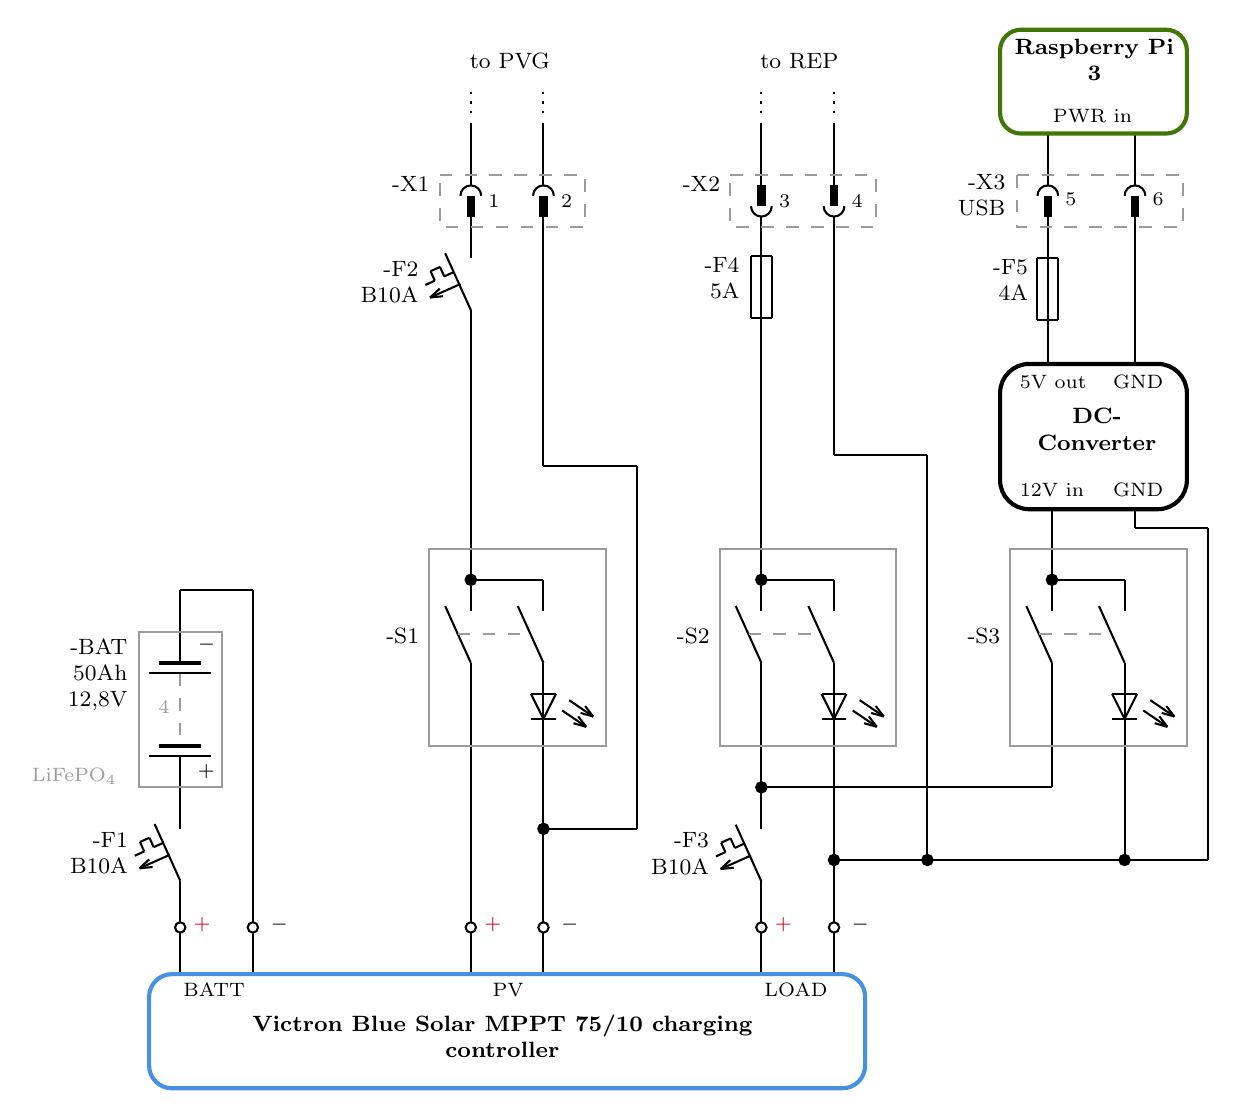
\begin{tikzpicture}[x=0.75pt,y=0.75pt,yscale=-1,xscale=1]
%uncomment if require: \path (0,819); %set diagram left start at 0, and has height of 819

%Straight Lines [id:da6045487236887532] 
\draw    (110,695) -- (110,715) ;
%Straight Lines [id:da8087426483801843] 
\draw    (110,650) -- (110,670) ;
%Straight Lines [id:da8582664692403452] 
\draw    (377.65,562.66) -- (390,590) ;
%Straight Lines [id:da45947571472796644] 
\draw    (390,550) -- (390,565) ;
%Shape: Circle [id:dp8494279940553138] 
\draw  [fill={rgb, 255:red, 0; green, 0; blue, 0 }  ,fill opacity=1 ] (387.5,550) .. controls (387.5,548.62) and (388.62,547.5) .. (390,547.5) .. controls (391.38,547.5) and (392.5,548.62) .. (392.5,550) .. controls (392.5,551.38) and (391.38,552.5) .. (390,552.5) .. controls (388.62,552.5) and (387.5,551.38) .. (387.5,550) -- cycle ;
%Straight Lines [id:da9379830792528405] 
\draw    (390,550) -- (425,550) ;
%Straight Lines [id:da11204638600738326] 
\draw    (412.65,562.66) -- (425,590) ;
%Straight Lines [id:da8198079156830071] 
\draw    (425,550) -- (425,565) ;
%Straight Lines [id:da9709654105257282] 
\draw [color={rgb, 255:red, 155; green, 155; blue, 155 }  ,draw opacity=1 ] [dash pattern={on 4.5pt off 4.5pt}]  (383.83,576.33) -- (418.83,576.33) ;
%Straight Lines [id:da4406437098546989] 
\draw    (437.37,608) -- (448.95,615.87) ;
%Straight Lines [id:da5984639010486943] 
\draw    (448.95,615.87) -- (442.87,614.15) ;
%Straight Lines [id:da05242179546825909] 
\draw    (448.95,615.87) -- (445.11,610.84) ;
%Straight Lines [id:da03867943479010427] 
\draw    (434,612.96) -- (445.58,620.83) ;
%Straight Lines [id:da3784375658363819] 
\draw    (445.58,620.83) -- (439.49,619.11) ;
%Straight Lines [id:da10650663928320747] 
\draw    (445.58,620.83) -- (441.74,615.8) ;
%Straight Lines [id:da21253577517529276] 
\draw    (390,535) -- (390,550) ;
%Straight Lines [id:da35682397636352925] 
\draw    (425,590) -- (425,630) ;
%Straight Lines [id:da6087198215051832] 
\draw    (425,605) -- (419,605) ;
%Straight Lines [id:da1327541924284974] 
\draw    (431,605) -- (425,605) ;
%Straight Lines [id:da3477318152682538] 
\draw    (425,617) -- (419,617) ;
%Straight Lines [id:da5388714005450448] 
\draw    (431,617) -- (425,617) ;
%Straight Lines [id:da45545990971532424] 
\draw    (419,605) -- (425,617) ;
%Straight Lines [id:da6636904871804508] 
\draw    (425,617) -- (431,605) ;
%Straight Lines [id:da8527469668539813] 
\draw    (390,590) -- (390,630) ;
%Straight Lines [id:da7447466868999879] 
\draw    (390,695) -- (390,715) ;
%Straight Lines [id:da781957856780034] 
\draw    (390,650) -- (390,670) ;
%Straight Lines [id:da9660919188574675] 
\draw    (237.65,562.66) -- (250,590) ;
%Straight Lines [id:da6074395418040595] 
\draw    (250,550) -- (250,565) ;
%Shape: Circle [id:dp9079157732157477] 
\draw  [fill={rgb, 255:red, 0; green, 0; blue, 0 }  ,fill opacity=1 ] (247.5,550) .. controls (247.5,548.62) and (248.62,547.5) .. (250,547.5) .. controls (251.38,547.5) and (252.5,548.62) .. (252.5,550) .. controls (252.5,551.38) and (251.38,552.5) .. (250,552.5) .. controls (248.62,552.5) and (247.5,551.38) .. (247.5,550) -- cycle ;
%Straight Lines [id:da30373671566038385] 
\draw    (250,550) -- (285,550) ;
%Straight Lines [id:da8970508873642955] 
\draw    (272.65,562.66) -- (285,590) ;
%Straight Lines [id:da7659644393479124] 
\draw    (285,550) -- (285,565) ;
%Straight Lines [id:da08340396961097585] 
\draw [color={rgb, 255:red, 155; green, 155; blue, 155 }  ,draw opacity=1 ] [dash pattern={on 4.5pt off 4.5pt}]  (243.83,576.33) -- (278.83,576.33) ;
%Straight Lines [id:da7022147637544038] 
\draw    (297.37,608) -- (308.95,615.87) ;
%Straight Lines [id:da0764773735026596] 
\draw    (308.95,615.87) -- (302.87,614.15) ;
%Straight Lines [id:da44832120210981063] 
\draw    (308.95,615.87) -- (305.11,610.84) ;
%Straight Lines [id:da6526028841069826] 
\draw    (294,612.96) -- (305.58,620.83) ;
%Straight Lines [id:da6507660687441759] 
\draw    (305.58,620.83) -- (299.49,619.11) ;
%Straight Lines [id:da3754400469273893] 
\draw    (305.58,620.83) -- (301.74,615.8) ;
%Straight Lines [id:da2708393949170931] 
\draw    (250,535) -- (250,550) ;
%Straight Lines [id:da6240610752921043] 
\draw    (285,590) -- (285,630) ;
%Straight Lines [id:da8049652672008647] 
\draw    (285,605) -- (279,605) ;
%Straight Lines [id:da7379771383648002] 
\draw    (291,605) -- (285,605) ;
%Straight Lines [id:da8869453156089939] 
\draw    (285,617) -- (279,617) ;
%Straight Lines [id:da7435846187752939] 
\draw    (291,617) -- (285,617) ;
%Straight Lines [id:da615016788311137] 
\draw    (279,605) -- (285,617) ;
%Straight Lines [id:da6488268995665789] 
\draw    (285,617) -- (291,605) ;
%Straight Lines [id:da5943328902614433] 
\draw    (250,590) -- (250,630) ;
%Straight Lines [id:da25421541890667876] 
\draw    (237.65,392.66) -- (250,420) ;
%Straight Lines [id:da18896174609521244] 
\draw    (237.21,403.83) -- (241.77,401.77) ;
%Straight Lines [id:da8843882614062888] 
\draw    (230.6,401.33) -- (235.16,399.27) ;
%Straight Lines [id:da9702160555624855] 
\draw    (237.21,403.83) -- (235.16,399.27) ;
%Straight Lines [id:da16220285906727772] 
\draw    (232.66,405.89) -- (230.6,401.33) ;
%Straight Lines [id:da8185940982825655] 
\draw    (228.1,407.94) -- (232.66,405.89) ;
%Straight Lines [id:da5227549662131044] 
\draw    (250,375) -- (250,395) ;
%Straight Lines [id:da8132646700506851] 
\draw    (230.39,414) -- (245,407.49) ;
%Straight Lines [id:da3010763046079674] 
\draw    (235.05,409.73) -- (230.39,414) ;
%Straight Lines [id:da007640196399169241] 
\draw    (236.68,413.38) -- (230.39,414) ;
%Straight Lines [id:da10235742797497815] 
\draw    (250,630) -- (250,715) ;
%Straight Lines [id:da34716144349513156] 
\draw    (285,630) -- (285,715) ;
%Shape: Circle [id:dp314607867217201] 
\draw  [fill={rgb, 255:red, 0; green, 0; blue, 0 }  ,fill opacity=1 ] (282.5,670) .. controls (282.5,668.62) and (283.62,667.5) .. (285,667.5) .. controls (286.38,667.5) and (287.5,668.62) .. (287.5,670) .. controls (287.5,671.38) and (286.38,672.5) .. (285,672.5) .. controls (283.62,672.5) and (282.5,671.38) .. (282.5,670) -- cycle ;
%Straight Lines [id:da28477361830913206] 
\draw    (285,670) -- (330,670) ;
%Straight Lines [id:da09232950946566088] 
\draw    (330,670) -- (330,495) ;
%Straight Lines [id:da13780659251530203] 
\draw    (285,495) -- (330,495) ;
%Straight Lines [id:da7851445656752061] 
\draw [line width=3]    (250,365) -- (250,375) ;
%Shape: Circle [id:dp6899792380181562] 
\draw   (107.5,717.5) .. controls (107.5,716.12) and (108.62,715) .. (110,715) .. controls (111.38,715) and (112.5,716.12) .. (112.5,717.5) .. controls (112.5,718.88) and (111.38,720) .. (110,720) .. controls (108.62,720) and (107.5,718.88) .. (107.5,717.5) -- cycle ;
%Straight Lines [id:da47366118482865205] 
\draw    (145,720) -- (145,740) ;
%Straight Lines [id:da8468122562252522] 
\draw    (110,720) -- (110,740) ;
%Shape: Circle [id:dp035454590154937904] 
\draw   (142.5,717.5) .. controls (142.5,716.12) and (143.62,715) .. (145,715) .. controls (146.38,715) and (147.5,716.12) .. (147.5,717.5) .. controls (147.5,718.88) and (146.38,720) .. (145,720) .. controls (143.62,720) and (142.5,718.88) .. (142.5,717.5) -- cycle ;
%Straight Lines [id:da6492577157597839] 
\draw [line width=0.75]    (95,635) -- (125,635) ;
%Straight Lines [id:da3387989968134515] 
\draw [color={rgb, 255:red, 155; green, 155; blue, 155 }  ,draw opacity=1 ] [dash pattern={on 4.5pt off 4.5pt}]  (110,595) -- (110,630) ;
%Straight Lines [id:da6269085784209374] 
\draw    (145,715) -- (145,555) ;
%Straight Lines [id:da5418431146259968] 
\draw [line width=1.5]    (100,630) -- (120,630) ;
%Straight Lines [id:da2961999630078498] 
\draw [line width=0.75]    (95,595) -- (125,595) ;
%Straight Lines [id:da3887851996750402] 
\draw [line width=1.5]    (100,590) -- (120,590) ;
%Straight Lines [id:da5555796206150274] 
\draw    (110,635) -- (110,650) ;
%Straight Lines [id:da048935027069065384] 
\draw    (110,575) -- (110,590) ;
%Straight Lines [id:da30715757282137335] 
\draw    (145,555) -- (110,555) ;
%Straight Lines [id:da5029961778247691] 
\draw    (110,555) -- (110,575) ;
%Shape: Arc [id:dp12633069475347658] 
\draw  [draw opacity=0] (395,370) .. controls (395,370) and (395,370) .. (395,370) .. controls (395,370) and (395,370) .. (395,370) .. controls (395,372.76) and (392.76,375) .. (390,375) .. controls (387.24,375) and (385,372.76) .. (385,370) -- (390,370) -- cycle ; \draw   (395,370) .. controls (395,370) and (395,370) .. (395,370) .. controls (395,370) and (395,370) .. (395,370) .. controls (395,372.76) and (392.76,375) .. (390,375) .. controls (387.24,375) and (385,372.76) .. (385,370) ;
%Straight Lines [id:da029085655956979428] 
\draw [line width=3]    (285,365) -- (285,375) ;
%Shape: Arc [id:dp6387147329073852] 
\draw  [draw opacity=0] (430,370) .. controls (430,370) and (430,370) .. (430,370) .. controls (430,370) and (430,370) .. (430,370) .. controls (430,372.76) and (427.76,375) .. (425,375) .. controls (422.24,375) and (420,372.76) .. (420,370) -- (425,370) -- cycle ; \draw   (430,370) .. controls (430,370) and (430,370) .. (430,370) .. controls (430,370) and (430,370) .. (430,370) .. controls (430,372.76) and (427.76,375) .. (425,375) .. controls (422.24,375) and (420,372.76) .. (420,370) ;
%Straight Lines [id:da7300180336801758] 
\draw    (385,424) -- (395,424) ;
%Straight Lines [id:da549626539382917] 
\draw    (385,394) -- (395,394) ;
%Straight Lines [id:da14279688282187109] 
\draw    (385,394) -- (385,424) ;
%Straight Lines [id:da3447163030596341] 
\draw    (395,394) -- (395,424) ;
%Shape: Circle [id:dp5086380236446248] 
\draw  [fill={rgb, 255:red, 0; green, 0; blue, 0 }  ,fill opacity=1 ] (422.5,685) .. controls (422.5,683.62) and (423.62,682.5) .. (425,682.5) .. controls (426.38,682.5) and (427.5,683.62) .. (427.5,685) .. controls (427.5,686.38) and (426.38,687.5) .. (425,687.5) .. controls (423.62,687.5) and (422.5,686.38) .. (422.5,685) -- cycle ;
%Shape: Circle [id:dp7343870876537575] 
\draw  [fill={rgb, 255:red, 0; green, 0; blue, 0 }  ,fill opacity=1 ] (387.5,650) .. controls (387.5,648.62) and (388.62,647.5) .. (390,647.5) .. controls (391.38,647.5) and (392.5,648.62) .. (392.5,650) .. controls (392.5,651.38) and (391.38,652.5) .. (390,652.5) .. controls (388.62,652.5) and (387.5,651.38) .. (387.5,650) -- cycle ;
%Straight Lines [id:da9947564306759737] 
\draw    (390,630) -- (390,650) ;
%Straight Lines [id:da04267171410214621] 
\draw    (517.65,562.66) -- (530,590) ;
%Straight Lines [id:da34260340218397145] 
\draw    (530,550) -- (530,565) ;
%Shape: Circle [id:dp9118380193654758] 
\draw  [fill={rgb, 255:red, 0; green, 0; blue, 0 }  ,fill opacity=1 ] (527.5,550) .. controls (527.5,548.62) and (528.62,547.5) .. (530,547.5) .. controls (531.38,547.5) and (532.5,548.62) .. (532.5,550) .. controls (532.5,551.38) and (531.38,552.5) .. (530,552.5) .. controls (528.62,552.5) and (527.5,551.38) .. (527.5,550) -- cycle ;
%Straight Lines [id:da36678432079339074] 
\draw    (530,550) -- (565,550) ;
%Straight Lines [id:da2194266974250345] 
\draw    (552.65,562.66) -- (565,590) ;
%Straight Lines [id:da9840656063211173] 
\draw    (565,550) -- (565,565) ;
%Straight Lines [id:da8595646767861336] 
\draw [color={rgb, 255:red, 155; green, 155; blue, 155 }  ,draw opacity=1 ] [dash pattern={on 4.5pt off 4.5pt}]  (523.83,576.33) -- (558.83,576.33) ;
%Straight Lines [id:da15163171347844262] 
\draw    (577.37,608) -- (588.95,615.87) ;
%Straight Lines [id:da9196970545090257] 
\draw    (588.95,615.87) -- (582.87,614.15) ;
%Straight Lines [id:da3063314574752225] 
\draw    (588.95,615.87) -- (585.11,610.84) ;
%Straight Lines [id:da6975056042812295] 
\draw    (574,612.96) -- (585.58,620.83) ;
%Straight Lines [id:da054383032504933926] 
\draw    (585.58,620.83) -- (579.49,619.11) ;
%Straight Lines [id:da28434109299540156] 
\draw    (585.58,620.83) -- (581.74,615.8) ;
%Straight Lines [id:da22683364116436477] 
\draw    (530,535) -- (530,550) ;
%Straight Lines [id:da7050825089011707] 
\draw    (565,590) -- (565,630) ;
%Straight Lines [id:da21917911924144184] 
\draw    (565,605) -- (559,605) ;
%Straight Lines [id:da361649133281567] 
\draw    (571,605) -- (565,605) ;
%Straight Lines [id:da35886660187596586] 
\draw    (565,617) -- (559,617) ;
%Straight Lines [id:da5846400944890127] 
\draw    (571,617) -- (565,617) ;
%Straight Lines [id:da16363774592191427] 
\draw    (559,605) -- (565,617) ;
%Straight Lines [id:da8495558971534367] 
\draw    (565,617) -- (571,605) ;
%Straight Lines [id:da9705301356465246] 
\draw    (530,590) -- (530,630) ;
%Straight Lines [id:da94488276559975] 
\draw    (530,630) -- (530,650) ;
%Straight Lines [id:da6569007196192038] 
\draw    (390,650) -- (530,650) ;
%Straight Lines [id:da07957354820917795] 
\draw    (425,630) -- (425,668) -- (425,715) ;
%Straight Lines [id:da7588862768357891] 
\draw    (425,685) -- (565,685) ;
%Straight Lines [id:da7674253072712494] 
\draw    (565,630) -- (565,685) ;
%Straight Lines [id:da8866365135237142] 
\draw    (390,375) -- (390,535) ;
%Straight Lines [id:da8519154963271058] 
\draw    (533,395) -- (533,425) ;
%Straight Lines [id:da15281292683015657] 
\draw    (528,375) -- (528,445) ;
%Straight Lines [id:da7758273163735636] 
\draw    (285,720) -- (285,740) ;
%Straight Lines [id:da9301661325681598] 
\draw    (250,720) -- (250,740) ;
%Straight Lines [id:da6182430885473893] 
\draw    (425,720) -- (425,740) ;
%Straight Lines [id:da09806610463552223] 
\draw    (390,720) -- (390,740) ;
%Straight Lines [id:da5284630296909336] 
\draw    (470,685) -- (470,490) ;
%Straight Lines [id:da7560903430233721] 
\draw    (425,490) -- (470,490) ;
%Straight Lines [id:da7794407016175966] 
\draw    (425,375) -- (425,490) ;
%Shape: Circle [id:dp23063185673707154] 
\draw  [fill={rgb, 255:red, 0; green, 0; blue, 0 }  ,fill opacity=1 ] (467.5,685) .. controls (467.5,683.62) and (468.62,682.5) .. (470,682.5) .. controls (471.38,682.5) and (472.5,683.62) .. (472.5,685) .. controls (472.5,686.38) and (471.38,687.5) .. (470,687.5) .. controls (468.62,687.5) and (467.5,686.38) .. (467.5,685) -- cycle ;
%Straight Lines [id:da7690431263950712] 
\draw    (530,515) -- (530,535) ;
%Straight Lines [id:da7126295417227146] 
\draw    (570,515) -- (570,525) ;
%Straight Lines [id:da39047551968710303] 
\draw    (570,525) -- (605,525) ;
%Straight Lines [id:da562170190014285] 
\draw    (605,685) -- (605,525) ;
%Shape: Circle [id:dp1979323470578791] 
\draw  [fill={rgb, 255:red, 0; green, 0; blue, 0 }  ,fill opacity=1 ] (562.5,685) .. controls (562.5,683.62) and (563.62,682.5) .. (565,682.5) .. controls (566.38,682.5) and (567.5,683.62) .. (567.5,685) .. controls (567.5,686.38) and (566.38,687.5) .. (565,687.5) .. controls (563.62,687.5) and (562.5,686.38) .. (562.5,685) -- cycle ;
%Straight Lines [id:da7082116641337399] 
\draw    (565,685) -- (605,685) ;
%Straight Lines [id:da9591158667779314] 
\draw    (570,375) -- (570,445) ;
%Shape: Arc [id:dp12927742122754227] 
\draw  [draw opacity=0] (245,365) .. controls (245,365) and (245,365) .. (245,365) .. controls (245,365) and (245,365) .. (245,365) .. controls (245,362.24) and (247.24,360) .. (250,360) .. controls (252.76,360) and (255,362.24) .. (255,365) -- (250,365) -- cycle ; \draw   (245,365) .. controls (245,365) and (245,365) .. (245,365) .. controls (245,365) and (245,365) .. (245,365) .. controls (245,362.24) and (247.24,360) .. (250,360) .. controls (252.76,360) and (255,362.24) .. (255,365) ;
%Shape: Arc [id:dp9619689149899326] 
\draw  [draw opacity=0] (280,365) .. controls (280,365) and (280,365) .. (280,365) .. controls (280,365) and (280,365) .. (280,365) .. controls (280,362.24) and (282.24,360) .. (285,360) .. controls (287.76,360) and (290,362.24) .. (290,365) -- (285,365) -- cycle ; \draw   (280,365) .. controls (280,365) and (280,365) .. (280,365) .. controls (280,365) and (280,365) .. (280,365) .. controls (280,362.24) and (282.24,360) .. (285,360) .. controls (287.76,360) and (290,362.24) .. (290,365) ;
%Straight Lines [id:da04744516103344654] 
\draw [line width=3]    (390,360) -- (390,370) ;
%Straight Lines [id:da10347567503749389] 
\draw [line width=3]    (425,360) -- (425,370) ;
%Straight Lines [id:da006327163323699647] 
\draw    (250,330) -- (250,360) ;
%Straight Lines [id:da4125490721764107] 
\draw  [dash pattern={on 0.84pt off 2.51pt}]  (250,315) -- (250,325) ;
%Straight Lines [id:da7992654613315551] 
\draw    (285,330) -- (285,360) ;
%Straight Lines [id:da8169675414190176] 
\draw  [dash pattern={on 0.84pt off 2.51pt}]  (285,315) -- (285,325) ;
%Straight Lines [id:da12965980010822298] 
\draw    (390,330) -- (390,360) ;
%Straight Lines [id:da511508279901864] 
\draw  [dash pattern={on 0.84pt off 2.51pt}]  (390,315) -- (390,325) ;
%Straight Lines [id:da359939455942329] 
\draw    (425,330) -- (425,360) ;
%Straight Lines [id:da5754392508412918] 
\draw  [dash pattern={on 0.84pt off 2.51pt}]  (425,315) -- (425,325) ;
%Straight Lines [id:da8751948100537181] 
\draw [line width=3]    (528,365) -- (528,375) ;
%Straight Lines [id:da23535481794391266] 
\draw [line width=3]    (570,365) -- (570,375) ;
%Shape: Arc [id:dp52709460152225] 
\draw  [draw opacity=0] (523,365) .. controls (523,365) and (523,365) .. (523,365) .. controls (523,365) and (523,365) .. (523,365) .. controls (523,362.24) and (525.24,360) .. (528,360) .. controls (530.76,360) and (533,362.24) .. (533,365) -- (528,365) -- cycle ; \draw   (523,365) .. controls (523,365) and (523,365) .. (523,365) .. controls (523,365) and (523,365) .. (523,365) .. controls (523,362.24) and (525.24,360) .. (528,360) .. controls (530.76,360) and (533,362.24) .. (533,365) ;
%Shape: Arc [id:dp5986472781356484] 
\draw  [draw opacity=0] (565,365) .. controls (565,365) and (565,365) .. (565,365) .. controls (565,365) and (565,365) .. (565,365) .. controls (565,362.24) and (567.24,360) .. (570,360) .. controls (572.76,360) and (575,362.24) .. (575,365) -- (570,365) -- cycle ; \draw   (565,365) .. controls (565,365) and (565,365) .. (565,365) .. controls (565,365) and (565,365) .. (565,365) .. controls (565,362.24) and (567.24,360) .. (570,360) .. controls (572.76,360) and (575,362.24) .. (575,365) ;
%Straight Lines [id:da6970901106745506] 
\draw    (570,335) -- (570,360) ;
%Straight Lines [id:da8240417212964364] 
\draw    (528,335) -- (528,360) ;
%Straight Lines [id:da8981631423488339] 
\draw    (250,420) -- (250,535) ;
%Straight Lines [id:da3698727384717244] 
\draw    (285,375) -- (285,495) ;
%Shape: Rectangle [id:dp05337640820618983] 
\draw  [color={rgb, 255:red, 155; green, 155; blue, 155 }  ,draw opacity=1 ] (90,575) -- (130,575) -- (130,650) -- (90,650) -- cycle ;
%Rounded Rect [id:dp3749474500303014] 
\draw  [color={rgb, 255:red, 74; green, 144; blue, 226 }  ,draw opacity=1 ][line width=1.5]  (95,751) .. controls (95,744.92) and (99.92,740) .. (106,740) -- (429,740) .. controls (435.08,740) and (440,744.92) .. (440,751) -- (440,784) .. controls (440,790.08) and (435.08,795) .. (429,795) -- (106,795) .. controls (99.92,795) and (95,790.08) .. (95,784) -- cycle ;
%Shape: Rectangle [id:dp22986963428559748] 
\draw  [color={rgb, 255:red, 155; green, 155; blue, 155 }  ,draw opacity=1 ] (230,535) -- (315,535) -- (315,630) -- (230,630) -- cycle ;
%Shape: Rectangle [id:dp9538291811828312] 
\draw  [color={rgb, 255:red, 155; green, 155; blue, 155 }  ,draw opacity=1 ] (370,535) -- (455,535) -- (455,630) -- (370,630) -- cycle ;
%Shape: Rectangle [id:dp0001839428435912449] 
\draw  [color={rgb, 255:red, 155; green, 155; blue, 155 }  ,draw opacity=1 ] (510,535) -- (595,535) -- (595,630) -- (510,630) -- cycle ;
%Rounded Rect [id:dp6772567415083697] 
\draw  [line width=1.5]  (505,460) .. controls (505,452.27) and (511.27,446) .. (519,446) -- (581,446) .. controls (588.73,446) and (595,452.27) .. (595,460) -- (595,502) .. controls (595,509.73) and (588.73,516) .. (581,516) -- (519,516) .. controls (511.27,516) and (505,509.73) .. (505,502) -- cycle ;
%Shape: Rectangle [id:dp13677331896440492] 
\draw  [color={rgb, 255:red, 155; green, 155; blue, 155 }  ,draw opacity=1 ][dash pattern={on 4.5pt off 4.5pt}] (375,355) -- (445,355) -- (445,380) -- (375,380) -- cycle ;
%Shape: Rectangle [id:dp3588933470182385] 
\draw  [color={rgb, 255:red, 155; green, 155; blue, 155 }  ,draw opacity=1 ][dash pattern={on 4.5pt off 4.5pt}] (235,355) -- (305,355) -- (305,380) -- (235,380) -- cycle ;
%Shape: Circle [id:dp8175441348603898] 
\draw   (247.5,717.5) .. controls (247.5,716.12) and (248.62,715) .. (250,715) .. controls (251.38,715) and (252.5,716.12) .. (252.5,717.5) .. controls (252.5,718.88) and (251.38,720) .. (250,720) .. controls (248.62,720) and (247.5,718.88) .. (247.5,717.5) -- cycle ;
%Shape: Circle [id:dp4775207272259603] 
\draw   (387.5,717.5) .. controls (387.5,716.12) and (388.62,715) .. (390,715) .. controls (391.38,715) and (392.5,716.12) .. (392.5,717.5) .. controls (392.5,718.88) and (391.38,720) .. (390,720) .. controls (388.62,720) and (387.5,718.88) .. (387.5,717.5) -- cycle ;
%Shape: Circle [id:dp9698857310943421] 
\draw   (282.5,717.5) .. controls (282.5,716.12) and (283.62,715) .. (285,715) .. controls (286.38,715) and (287.5,716.12) .. (287.5,717.5) .. controls (287.5,718.88) and (286.38,720) .. (285,720) .. controls (283.62,720) and (282.5,718.88) .. (282.5,717.5) -- cycle ;
%Shape: Circle [id:dp0060774518425563695] 
\draw   (422.5,717.5) .. controls (422.5,716.12) and (423.62,715) .. (425,715) .. controls (426.38,715) and (427.5,716.12) .. (427.5,717.5) .. controls (427.5,718.88) and (426.38,720) .. (425,720) .. controls (423.62,720) and (422.5,718.88) .. (422.5,717.5) -- cycle ;
%Straight Lines [id:da9351882313390889] 
\draw    (97.65,667.66) -- (110,695) ;
%Straight Lines [id:da5194752510301774] 
\draw    (97.21,678.83) -- (101.77,676.77) ;
%Straight Lines [id:da7220617602483184] 
\draw    (90.6,676.33) -- (95.16,674.27) ;
%Straight Lines [id:da24308342963349783] 
\draw    (97.21,678.83) -- (95.16,674.27) ;
%Straight Lines [id:da2559444640763633] 
\draw    (92.66,680.89) -- (90.6,676.33) ;
%Straight Lines [id:da46670151165536833] 
\draw    (88.1,682.94) -- (92.66,680.89) ;
%Straight Lines [id:da5006061451785055] 
\draw    (90.39,689) -- (105,682.49) ;
%Straight Lines [id:da018190616723821496] 
\draw    (95.05,684.73) -- (90.39,689) ;
%Straight Lines [id:da05443186004578027] 
\draw    (96.68,688.38) -- (90.39,689) ;
%Straight Lines [id:da7996764091693653] 
\draw    (523,425) -- (533,425) ;
%Straight Lines [id:da029180202518775067] 
\draw    (523,395) -- (523,425) ;
%Straight Lines [id:da3003961162833264] 
\draw    (523,395) -- (533,395) ;
%Straight Lines [id:da5535657777248622] 
\draw    (377.65,668) -- (390,695.34) ;
%Straight Lines [id:da28100437921667276] 
\draw    (377.21,679.17) -- (381.77,677.11) ;
%Straight Lines [id:da8268331410120646] 
\draw    (370.6,676.67) -- (375.16,674.61) ;
%Straight Lines [id:da5593433507999295] 
\draw    (377.21,679.17) -- (375.16,674.61) ;
%Straight Lines [id:da8385823416593714] 
\draw    (372.66,681.23) -- (370.6,676.67) ;
%Straight Lines [id:da9041721517779324] 
\draw    (368.1,683.29) -- (372.66,681.23) ;
%Straight Lines [id:da06366421356292284] 
\draw    (370.39,689.34) -- (385,682.83) ;
%Straight Lines [id:da6819360673702595] 
\draw    (375.05,685.07) -- (370.39,689.34) ;
%Straight Lines [id:da3321669007849293] 
\draw    (376.68,688.73) -- (370.39,689.34) ;
%Shape: Rectangle [id:dp27771694740825015] 
\draw  [color={rgb, 255:red, 155; green, 155; blue, 155 }  ,draw opacity=1 ][dash pattern={on 4.5pt off 4.5pt}] (513,355) -- (593,355) -- (593,380) -- (513,380) -- cycle ;
%Rounded Rect [id:dp2840095531764171] 
\draw  [color={rgb, 255:red, 65; green, 117; blue, 5 }  ,draw opacity=1 ][line width=1.5]  (505,295) .. controls (505,289.48) and (509.48,285) .. (515,285) -- (585,285) .. controls (590.52,285) and (595,289.48) .. (595,295) -- (595,325) .. controls (595,330.52) and (590.52,335) .. (585,335) -- (515,335) .. controls (509.48,335) and (505,330.52) .. (505,325) -- cycle ;

% Text Node
\draw (343,572) node [anchor=north west][inner sep=0.75pt]  [font=\footnotesize] [align=left] {\begin{minipage}[lt]{15.427500000000002pt}\setlength\topsep{0pt}
\begin{flushright}
\mbox{-}S2
\end{flushright}

\end{minipage}};
% Text Node
\draw (257,363) node [anchor=north west][inner sep=0.75pt]  [font=\scriptsize] [align=left] {1};
% Text Node
\draw (292,363) node [anchor=north west][inner sep=0.75pt]  [font=\scriptsize] [align=left] {2};
% Text Node
\draw (132,758) node [anchor=north west][inner sep=0.75pt]  [font=\footnotesize] [align=left] {\begin{minipage}[lt]{197.56108pt}\setlength\topsep{0pt}
\begin{center}
\textbf{Victron Blue Solar MPPT 75/10 charging controller}
\end{center}

\end{minipage}};
% Text Node
\draw (110,743) node [anchor=north west][inner sep=0.75pt]  [font=\scriptsize] [align=left] {BATT};
% Text Node
\draw (259,743) node [anchor=north west][inner sep=0.75pt]  [font=\scriptsize] [align=left] {PV};
% Text Node
\draw (390,743) node [anchor=north west][inner sep=0.75pt]  [font=\scriptsize] [align=left] {LOAD};
% Text Node
\draw (203,572) node [anchor=north west][inner sep=0.75pt]  [font=\footnotesize] [align=left] {\begin{minipage}[lt]{15.427500000000002pt}\setlength\topsep{0pt}
\begin{flushright}
\mbox{-}S1
\end{flushright}

\end{minipage}};
% Text Node
\draw (193,395) node [anchor=north west][inner sep=0.75pt]  [font=\footnotesize] [align=left] {\begin{minipage}[lt]{22.684392000000003pt}\setlength\topsep{0pt}
\begin{flushright}
\mbox{-}F2\\B10A
\end{flushright}

\end{minipage}};
% Text Node
\draw (98,607) node [anchor=north west][inner sep=0.75pt]  [font=\scriptsize,color={rgb, 255:red, 155; green, 155; blue, 155 }  ,opacity=1 ] [align=left] {4};
% Text Node
\draw (51,577) node [anchor=north west][inner sep=0.75pt]  [font=\footnotesize] [align=left] {\begin{minipage}[lt]{24.044392000000002pt}\setlength\topsep{0pt}
\begin{flushright}
\mbox{-}BAT\\50Ah\\12,8V
\end{flushright}

\end{minipage}};
% Text Node
\draw (397,363) node [anchor=north west][inner sep=0.75pt]  [font=\scriptsize] [align=left] {3};
% Text Node
\draw (432,363) node [anchor=north west][inner sep=0.75pt]  [font=\scriptsize] [align=left] {4};
% Text Node
\draw (358,393) node [anchor=north west][inner sep=0.75pt]  [font=\footnotesize] [align=left] {\begin{minipage}[lt]{14.96pt}\setlength\topsep{0pt}
\begin{flushright}
\mbox{-}F4\\5A
\end{flushright}

\end{minipage}};
% Text Node
\draw (483,572) node [anchor=north west][inner sep=0.75pt]  [font=\footnotesize] [align=left] {\begin{minipage}[lt]{15.427500000000002pt}\setlength\topsep{0pt}
\begin{flushright}
\mbox{-}S3
\end{flushright}

\end{minipage}};
% Text Node
\draw (513,466) node [anchor=north west][inner sep=0.75pt]  [font=\footnotesize] [align=left] {\begin{minipage}[lt]{55.77060800000001pt}\setlength\topsep{0pt}
\begin{center}
\textbf{DC-Converter}
\end{center}

\end{minipage}};
% Text Node
\draw (509,288) node [anchor=north west][inner sep=0.75pt]  [font=\footnotesize] [align=left] {\begin{minipage}[lt]{59.871892pt}\setlength\topsep{0pt}
\begin{center}
\textbf{Raspberry Pi 3}
\end{center}

\end{minipage}};
% Text Node
\draw (513,502) node [anchor=north west][inner sep=0.75pt]  [font=\scriptsize] [align=left] {12V in};
% Text Node
\draw (558,450) node [anchor=north west][inner sep=0.75pt]  [font=\scriptsize] [align=left] {GND};
% Text Node
\draw (513,450) node [anchor=north west][inner sep=0.75pt]  [font=\scriptsize] [align=left] {5V out};
% Text Node
\draw (558,502) node [anchor=north west][inner sep=0.75pt]  [font=\scriptsize] [align=left] {GND};
% Text Node
\draw (248,295) node [anchor=north west][inner sep=0.75pt]  [font=\footnotesize] [align=left] {to PVG};
% Text Node
\draw (208,354) node [anchor=north west][inner sep=0.75pt]  [font=\footnotesize] [align=left] {\begin{minipage}[lt]{15.427500000000002pt}\setlength\topsep{0pt}
\begin{flushright}
\mbox{-}X1
\end{flushright}

\end{minipage}};
% Text Node
\draw (348,354) node [anchor=north west][inner sep=0.75pt]  [font=\footnotesize] [align=left] {\begin{minipage}[lt]{15.427500000000002pt}\setlength\topsep{0pt}
\begin{flushright}
\mbox{-}X2
\end{flushright}

\end{minipage}};
% Text Node
\draw (535,362) node [anchor=north west][inner sep=0.75pt]  [font=\scriptsize] [align=left] {5};
% Text Node
\draw (577,362) node [anchor=north west][inner sep=0.75pt]  [font=\scriptsize] [align=left] {6};
% Text Node
\draw (480,353) node [anchor=north west][inner sep=0.75pt]  [font=\footnotesize] [align=left] {\begin{minipage}[lt]{19.5075pt}\setlength\topsep{0pt}
\begin{flushright}
\mbox{-}X3\\USB
\end{flushright}

\end{minipage}};
% Text Node
\draw (529,322) node [anchor=north west][inner sep=0.75pt]  [font=\scriptsize] [align=left] {PWR in};
% Text Node
\draw (152,711.4) node [anchor=north west][inner sep=0.75pt]  [font=\scriptsize]  {$-$};
% Text Node
\draw (115,711.4) node [anchor=north west][inner sep=0.75pt]  [font=\scriptsize,color={rgb, 255:red, 208; green, 2; blue, 27 }  ,opacity=1 ]  {$+$};
% Text Node
\draw (255,711.4) node [anchor=north west][inner sep=0.75pt]  [font=\scriptsize,color={rgb, 255:red, 208; green, 2; blue, 27 }  ,opacity=1 ]  {$+$};
% Text Node
\draw (395,711.4) node [anchor=north west][inner sep=0.75pt]  [font=\scriptsize,color={rgb, 255:red, 208; green, 2; blue, 27 }  ,opacity=1 ]  {$+$};
% Text Node
\draw (292,711.4) node [anchor=north west][inner sep=0.75pt]  [font=\scriptsize]  {$-$};
% Text Node
\draw (432,711.4) node [anchor=north west][inner sep=0.75pt]  [font=\scriptsize]  {$-$};
% Text Node
\draw (117,637.4) node [anchor=north west][inner sep=0.75pt]  [font=\scriptsize,color={rgb, 255:red, 0; green, 0; blue, 0 }  ,opacity=1 ]  {$+$};
% Text Node
\draw (117,576.4) node [anchor=north west][inner sep=0.75pt]  [font=\scriptsize]  {$-$};
% Text Node
\draw (53,670) node [anchor=north west][inner sep=0.75pt]  [font=\footnotesize] [align=left] {\begin{minipage}[lt]{22.684392000000003pt}\setlength\topsep{0pt}
\begin{flushright}
\mbox{-}F1\\B10A
\end{flushright}

\end{minipage}};
% Text Node
\draw (497,394) node [anchor=north west][inner sep=0.75pt]  [font=\footnotesize] [align=left] {\begin{minipage}[lt]{14.96pt}\setlength\topsep{0pt}
\begin{flushright}
\mbox{-}F5\\4A
\end{flushright}

\end{minipage}};
% Text Node
\draw (333,670.34) node [anchor=north west][inner sep=0.75pt]  [font=\footnotesize] [align=left] {\begin{minipage}[lt]{22.684392000000003pt}\setlength\topsep{0pt}
\begin{flushright}
\mbox{-}F3\\B10A
\end{flushright}

\end{minipage}};
% Text Node
\draw (37,639.4) node [anchor=north west][inner sep=0.75pt]  [font=\scriptsize,color={rgb, 255:red, 0; green, 0; blue, 0 }  ,opacity=1 ]  {$\mathrm{\textcolor[rgb]{0.61,0.61,0.61}{LiFePO}\textcolor[rgb]{0.61,0.61,0.61}{_{4}}}$};
% Text Node
\draw (388,295) node [anchor=north west][inner sep=0.75pt]  [font=\footnotesize] [align=left] {to REP};


\end{tikzpicture}

	\caption{Circuit diagram of the battery box.}
	\label{fig:tikz_bvcr_battery_box_circuit_diagram}
\end{figure}

\section{Mission operations crew}
\subsection{System overview}
\subsection{Motorola Mototrbo DM 2600 mobile radio}

\section{Self-sufficient backup voice communication repeater}
\subsection{System overview}
\subsection{Motorola Mototrbo SLR 1000 repeater}
\subsection{Mechanical parts}

\section{Serenity's backup voice communication}
\subsection{System overview}
\subsection{Motorola Mototrbo SL 2600 handheld radio}

\section{Mission safety crew}
\subsection{System overview}
\subsection{Motorola Mototrbo SL 2600 handheld radio}

\section{Mission on-site support crew}
\subsection{System overview}
\subsection{Motorola Mototrbo DP 3601 handheld radio}